\chapter{Yield extraction}
\label{chap:prod:fitting}

Signal charm mesons can be distinguished from combinatorial background in the 
invariant mass distribution, as shown in \cref{fig:prod:sel:D0ToKpi:offline} 
for example.
However, the contributions from prompt and secondary charm are identical in the 
invariant mass, and so another distribution must be used to distinguish between 
the two sources of charm decays.

This analysis uses the logarithm of the \chisq\ of the \acl{IP}, \lnipchisq, to 
obtain the prompt charm yields.
The momentum vector of prompt charm should point back to the \ac{PV}, and so 
the \lnipchisq\ distribution is expected be centred around zero.
For secondary charm the \lnipchisq\ distribution is expected to peak at higher 
values.
This separation is exploited to distinguish between prompt and secondary charm, 
where the prompt signal yield in each \pTy\ bin is measured by a binned, 
extended maximum likelihood fit to the \lnipchisq\ distribution.
The prompt and secondary models in this fit are described analytically as 
peaking functions.
The combinatorial background is described by a non-parametric model taken from 
the data outside the signal peak in the mass distribution.
This background model is normalised in the \lnipchisq\ fit to the number of 
combinatorial background candidates in a signal window defined in the mass 
distribution, measured in a fit to the charm hadron mass spectrum.

For all cases but the \PDstarp\ measurement, it is the mass of the charm hadron 
that is used to discriminate all signal from combinatorial background.
For the \PDstarp\ measurement, the delta mass distribution is used instead, 
defined as the difference \deltam\ between the reconstructed \PDstarp\ mass and 
the reconstructed \PDzero mass
\begin{equation}
  \deltam = m(\PKminus\Ppiplus\Ppiplussoft) - m(\PKminus\Ppiplus).
  \label{eqn:prod:fitting:delta_mass}
\end{equation}
This has a nominal value of \SI{145.4}{\MeVcc}~\cite{PDG2014}.
The narrower signal peak allows for a better signal-to-background ratio.

\section{Signal-background discrimination}
\label{chap:prod:fitting:mass}

For each one-dimensional mass and \deltam\ fit, one PDF is defined per 
discriminatory species: signal and combinatorial background.
In both the mass and \deltam\ distributions, the prompt and secondary signal 
shapes are assumed to be identical, and for the \deltam\ fits the combinatorial 
background is assumed to be indistinguishable from random soft pion 
backgrounds, where a true \PDzero is combined with a random track in the event.
The total \ac{PDF} is constructed as the sum of the per-species \acp{PDF}, each $f_{s}$, 
each weighted by the respective yield $N_{s}$
\begin{align}
  f(m) &= \frac{1}{\sum_{\textnormal{s}} N_{\textnormal{s}}}
          \sum_{\textnormal{s}} N_{\textnormal{s}}
          f_{\textnormal{s}}(m),\\
  f(\deltam) &= \frac{1}{\sum_{\textnormal{s}} N_{\textnormal{s}}}
                \sum_{\textnormal{s}} N_{\textnormal{s}}
                f_{\textnormal{s}}(\deltam).
\end{align}

For every mass fit, the background PDF $f_{\textnormal{Bkg.}}(m)$ is taken to 
be a first-order polynomial, and the signal PDF $f_{\textnormal{Sig.}}(m)$ is 
dependent on the charm hadron candidate, with details given in 
Section~\ref{chap:prod:fitting:details}.
The combinatorial and random soft pion background in the \deltam\ fits are 
modelled as a single empirical threshold function of the (un-normalised) form
\begin{equation}
  % (dm - dm0)^A * exp(B*dm)
  % The exponential factor has been omitted, as we just set B = 0
  R(x; \deltam_{0}, A) = {(x - \deltam_{0})}^A,
\end{equation}
where $\deltam_{0}$ is the threshold value, fixed to the charged pion rest mass 
$m_{\Ppipm} = \SI{139.57}{\MeVcc}$~\cite{PDG2014}.
The signal PDF in \deltam\ is the sum of three normal distributions, sharing a 
common mean but allowed to have different widths.

One mass or \deltam\ PDF, $f(m)$ or $f(\deltam)$, is constructed per \pTy\ bin, 
and the likelihood is formed as the product of these such that each PDF is 
fitted simultaneously when the \ac{NLL} is minimised.

\section{Prompt-secondary discrimination}
\label{chap:prod:fitting:ipchisq}

The prompt and secondary signal distributions are modelled by continuous, 
parametric \acp{PDF}.
Rather than attempting to parameterise the combinatorial background 
distribution, a \acf{KDE} \ac{PDF}~\cite{Poluektov:2014rxa}, or `template', is 
created from a histogram of the \lnipchisq\ distribution in the lower and upper 
sidebands of the reconstructed charm hadron mass.
In the case of the \PDstarp measurements, the data in the upper sideband of the 
\deltam\ distribution are used instead.
This approach assumes that the mass and \lnipchisq\ are uncorrelated in the 
background sample, such that the \lnipchisq\ shape in the signal region is the 
same as that in the sidebands.

The signal region in each long-lived charm hadron mass distribution is defined 
as a \SI{40}{\MeVcc}-wide window centred on the nominal rest mass of the given 
charm hadron, taken to be \SI{1864.84}{\MeVcc}, \SI{1869.61}{\MeVcc}, and 
\SI{1968.30}{\MeVcc} for \PDzero, \PDplus, and \PDsplus~\cite{PDG2014}.
The lower sideband is a \SI{20}{\MeVcc}-wide window centred \SI{50}{\MeVcc} 
below the centre of the signal window, and the upper sideband is a 
\SI{20}{\MeVcc}-wide window centred \SI{50}{\MeVcc} above the centre of the 
signal window.
For the \PDstarp\ measurements, the signal region is defined as a window 
\SI{6}{\MeVcc} wide, centred on the nominal \deltam\ value of 
\SI{145.43}{\MeVcc}~\cite{PDG2014}.
The upper sideband, or just `sideband' as a lower sideband region is not 
defined in \deltam, is defined as the region from \SI{4.5}{\MeVcc} to 
\SI{9}{\MeVcc} above the centre of the signal region.
\Cref{fig:prod:fitting:regions_A,fig:prod:fitting:regions_B}
show the signal and sideband regions for each mode.

The integral of the \lnipchisq\ background template \ac{PDF} is 
Gaussian-constrained to the number of background candidates in the mass or 
\deltam\ signal region.
To avoid any complications due to correlations between the background template 
\ac{PDF} and the fitted data, only the data in signal region are used in the 
\lnipchisq\ fit.
For the \PDstarp\ measurements, this signal region requirement is made in both 
the \PDzero mass and the \deltam\ distributions.

For each one-dimensional \lnipchisq\ fit, one \ac{PDF} $f_{s}$ per 
discriminatory species is assigned: prompt signal, secondary signal, and 
combinatorial background.
The total \acp{PDF} are constructed as the sum of per-species \acp{PDF}, 
each weighted by the respective yield $N_{s}$
\begin{equation}
  f(\lnipchisq) = \frac{1}{\sum_{\textnormal{s}} N_{\textnormal{s}}}
                  \sum_{\text{s}} N_{\text{s}}
                  f_{\text{s}}(\lnipchisq).
\end{equation}
The constraint on the background yield \nbkg\ is applied by multiplying the 
likelihood by a normal distribution in \nbkg, whose mean is the number of 
background candidates measured by the mass fit and whose width is the 
uncertainty on that value.
This penalises the likelihood by reducing its value when the fitted \nbkg\ 
parameter is far away from the value found in the mass fit.

One \lnipchisq\ \ac{PDF} and background constraint is constructed per \pTy\ 
bin, and the likelihood is formed as the product of these such that each 
\ac{PDF} is fitted simultaneously when the negative log-likelihood is 
minimised.
The benefit of this construction is that some shape parameters can be shared 
across bins, reducing the uncertainty on the fit parameters.
Which parameters are shared across bins and which are fitted independently is 
dependent on the type of charm meson.
The shared and independent parameters are enumerated in 
\cref{chap:prod:fitting:details}.

The prompt signal model $H$ in the \lnipchisq\ distribution is a modified 
normal distribution, where the width is allowed to be asymmetric with respect 
to the mean, and the tails are described by exponential functions,
\begin{equation}
  H(x; \mu, \sigma, \epsilon, \rho_{L}, \rho_{R}) =
  \begin{cases}
    \exp\left(\frac{\rho_{L}^{2}}{2} + \rho_{L}\frac{x - \mu}{(1 - 
    \epsilon)\sigma}\right) & x < \mu - (\rho_{L}\sigma(1 - 
        \epsilon)), \\
    \exp\left(-\left(\frac{x - \mu}{\sqrt{2}\sigma(1 - 
    \epsilon)}\right)^{2}\right) & \mu - (\rho_{L}\sigma(1 - \epsilon)) 
          \leq x < \mu, \\
    \exp\left(-\left(\frac{x - \mu}{\sqrt{2}\sigma(1 + 
    \epsilon)}\right)^{2}\right) & \mu \leq x < \mu + (\rho_{R}\sigma(1 + 
          \epsilon)), \\
    \exp\left(\frac{\rho_{R}^{2}}{2} - \rho_{R}\frac{x - \mu}{(1 + 
    \epsilon)\sigma}\right) & x \geq \mu + (\rho_{R}\sigma(1 + 
        \epsilon)),
  \end{cases}
  \label{eqn:prod:fitting:ipchisq:signal_model}
\end{equation}
where the parameter $\mu$ is the mode of the distribution; $\sigma$ is the 
average of the left and right widths; $\epsilon$ is the asymmetry between the 
left and right widths; and $\rho_{L(R)}$ is the exponent for the left (right) 
tail.
The secondary signal distribution is modelled by a normal distribution.
These shapes are motivated by the \lnipchisq\ distributions for prompt and 
secondary signal decays observed in the \ac{MC} samples.

Given the large number of parameters to be fitted, some shape parameters in the 
prompt and secondary signal \lnipchisq\ \acp{PDF} are fixed to values obtained 
from `prefits' to the pure samples of prompt and secondary signal \ac{MC} 
described in \cref{chap:prod:data:mc}.
The set of parameters that is fixed is dependent on the charm meson species.

\section{Mode-specific details}
\label{chap:prod:fitting:details}

As different final states exhibit different features in the mass, \deltam, and 
\lnipchisq\ distributions, several aspects of the fits are different between 
modes.
This \lcnamecref{chap:prod:fitting:details} gives the list of parameters that 
are split between \pTy\ bins, and the list of parameters that are allowed to 
float after the \ac{MC} prefits, for each mode.

Initially, no knowledge is assumed on which parameters should be independent 
(to be `split') across the \pTy\ bins, nor of whether the \lnipchisq\ 
distribution is well-modelled by the \ac{MC}.
The chosen parameterisation is that which best describes the data.
For the mass fits, all parameters are initially fixed such that they are same 
across all \pTy\ bins, and are then split one by one when it is observed that a 
feature varies across the bins, such as the width of the signal peak.
All parameters of the \lnipchisq\ fits are first kept fixed to values found 
from the fits to the simulated data, and then individual parameters are floated 
if the total PDF does not model the data well.
Parameters are then split across \pTy\ bins in the same manner as in the mass 
fits.

\subsection{Fit details for \PDzero}
\label{chap:prod:fitting:details:D0ToKpi}

For the \DzToKpi\ mode, the signal shape in the mass fit is the sum of a normal 
and a Crystal Ball distribution~\cite{Skwarnicki:1986xj}, sharing a common mode 
but allowed to have different widths.
The Crystal Ball function $C$ is a normal distribution but with a power-law 
tail on one side, defined (un-normalised) as
\begin{equation}
  C(x; \mu, \sigma, \alpha, n) = \begin{cases}
    e^{-\frac{{(x - \mu)}^{2}}{2\sigma^{2}}}                          & \frac{x - \mu}{\sigma} > -\alpha, \\
    e^{-\frac{|\alpha|^{2}}{2}}
      {\left(\frac{n}{|\alpha|}\right)}^{n}
      {\left(\frac{n}{|\alpha|} - |\alpha| - \frac{x - \mu}{\sigma}\right)}^{-n} & \frac{x - \mu}{\sigma} \leq -\alpha,
  \end{cases}
  \label{eqn:prod:fitting:crystal_ball}
\end{equation}
where $\alpha$ defines where the power-law tail begins, in units of the width 
of the core Gaussian $\sigma$, and $n$ is the power law exponent.
The mode and width of the total signal \ac{PDF} are split across \pTy\ bins, as 
is the slope of the background \ac{PDF}.
The mode of the \lnipchisq\ prompt signal \ac{PDF} and the width of the 
secondary signal \ac{PDF} are also split across \pTy\ bins.
The mode and width of the prompt signal \lnipchisq\ \ac{PDF} and all parameters 
of the secondary signal \lnipchisq\ \ac{PDF} are floated in the fit to data, 
and all other \lnipchisq\ shape parameters are fixed to the values from 
\ac{MC}.

Prefits to the prompt signal and secondary signal \ac{MC} samples are given in 
\cref{fig:prod:fitting:prefits:D0ToKpi}.

\subsubsection*{Fit details for \PDplus}
\label{chap:prod:fitting:details:DpToKpipi}

For the \DpToKpipi\ mode, the signal shape in the mass fit is the sum of a 
normal and a Crystal Ball distribution, sharing a common mode but allowed to 
have different widths.
The mode of the signal mass \ac{PDF} as well as the width of the Crystal Ball 
component in the mass \ac{PDF} are split across \pTy\ bins, as is the slope of 
the background mass \ac{PDF}.
The mode of the \lnipchisq\ prompt signal and secondary signal distributions 
are split across \pTy\ bins.
The mode and tail parameters of the signal \lnipchisq\ \ac{PDF}, are floated 
during the fit to data, with all other shape parameters fixed to the values 
from \ac{MC}.

Prefits to the prompt signal and secondary signal data samples in \lnipchisq\ 
are given in \cref{fig:prod:fitting:prefits:DpToKpipi}.

\subsubsection*{Fit details for \PDsplus}
\label{chap:prod:fitting:details:DsToKKpi}

For the \DspTophipi\ mode, the signal shape in the mass fit is the sum of a two 
normal distributions, sharing a common mean but allowed to have different 
widths.
The mean and width of the signal mass \ac{PDF} and the slope of the background 
mass \ac{PDF}, along with the mode of the \lnipchisq\ prompt signal \ac{PDF}, 
are split across \pTy\ bins.
The mode of the prompt signal \lnipchisq\ \ac{PDF} and all parameters of the 
secondary \ac{PDF} are floated during the fit to data, with all other shape 
parameters fixed to the values from \ac{MC}.

Prefits to the prompt signal and secondary signal data samples in \lnipchisq\ 
are given in \cref{fig:prod:fitting:prefits:DsToKKpi}.

\subsubsection*{Fit details for \PDstarp}
\label{chap:prod:fitting:details:DstToD0pi}

For the \PDstarp-tagged \DzToKpi\ mode, the width of the widest component of 
the \deltam\ signal model, described in \cref{chap:prod:fitting:mass}, is split 
across \pTy\ bins, along with the mean of the prompt signal \lnipchisq\ 
\ac{PDF}.
The mean of the prompt signal \lnipchisq\ \ac{PDF} and all parameters of the 
secondary \ac{PDF} are floated during the fit to data, with all other shape 
parameters fixed to the values from \ac{MC}.

Prefits to the prompt signal and secondary signal data samples in \PDzero 
\lnipchisq\ are given in \cref{fig:prod:fitting:prefits:DstToD0pi_D0ToKpi}.

\subsection{Fit results}
\label{chap:prod:fitting:results}

For all fits, the covariance matrix is checked to be positive definite, and the 
goodness-of-fit within each \pTy\ bin is checked visually to ensure that the 
\ac{NLL} minimisation stopped at a sensible parameter value set.
Mass, \deltam, and \lnipchisq\ fits are given in 
\cref{fig:prod:fitting:D0ToKpi,fig:prod:fitting:DpToKpipi,fig:prod:fitting:DsToKKpi,fig:prod:fitting:DstToD0pi_D0ToKpi}, 
where the data and models shown are the sums of the data and models over all 
\pTy\ bins.
Prompt signal yields per \pTy\ bin are given in 
\cref{tab:prod:fitting:D0ToKpi,tab:prod:fitting:DpToKpipi,tab:prod:fitting:DsToKKpi,tab:prod:fitting:DstToD0pi_D0ToKpi}, 
and those integrated across all bins in \cref{tab:prod:fitting:integrated}.

The plots show that the models match the data well, but there are some 
significant discrepancies such as in 
\cref{fig:prod:fitting:DsToKKpi:ipchisq,fig:prod:fitting:DstToD0pi_D0ToKpi:delta_mass}.
However, the discrepancies in these integrated plots are exaggerations of those 
in the individual \pTy\ bin fits: they indicate that there is a consistent bias 
in the individual bins, but do not necessarily indicate that these are 
statistically significant.
For comparison, 
\cref{fig:prod:fitting:D0ToKpi:sig_bkg,fig:prod:fitting:DpToKpipi:sig_bkg,fig:prod:fitting:DsToKKpi:sig_bkg,fig:prod:fitting:DstToD0pi_D0ToKpi:sig_bkg} 
show the mass (or \deltam) and \lnipchisq\ fits for each meson in the \pTy\ bin 
with the highest prompt signal yield and in the \pTy\ bin with the highest 
combinatorial background yield.
These show that, in the individual \pTy\ bins, the fits model the data 
significantly better than the integrated plots would suggest, and also that the 
fit is flexible enough to model both high prompt signal and high combinatorial 
background datasets.
The effect on the cross-section measurements of mis-modelling will be discussed 
further in \cref{chap:prod:syst:fitting}.

In some \pTy\ bins, it is not possible to make a prompt signal yield 
measurement due to insufficient data in those bins.
At this stage in the analysis, a cross-section measurement in a bin is 
considered unfeasible if there is either no data (zero candidates), or if the 
prompt signal yield $N_{i} \pm \sigma_{N_{i}}$ in that bin as determined in the 
fit does not satisfy $N_{i} > 3\sigma_{N_{i}}$.

\begin{figure}
  \begin{subfigure}{0.5\textwidth}
    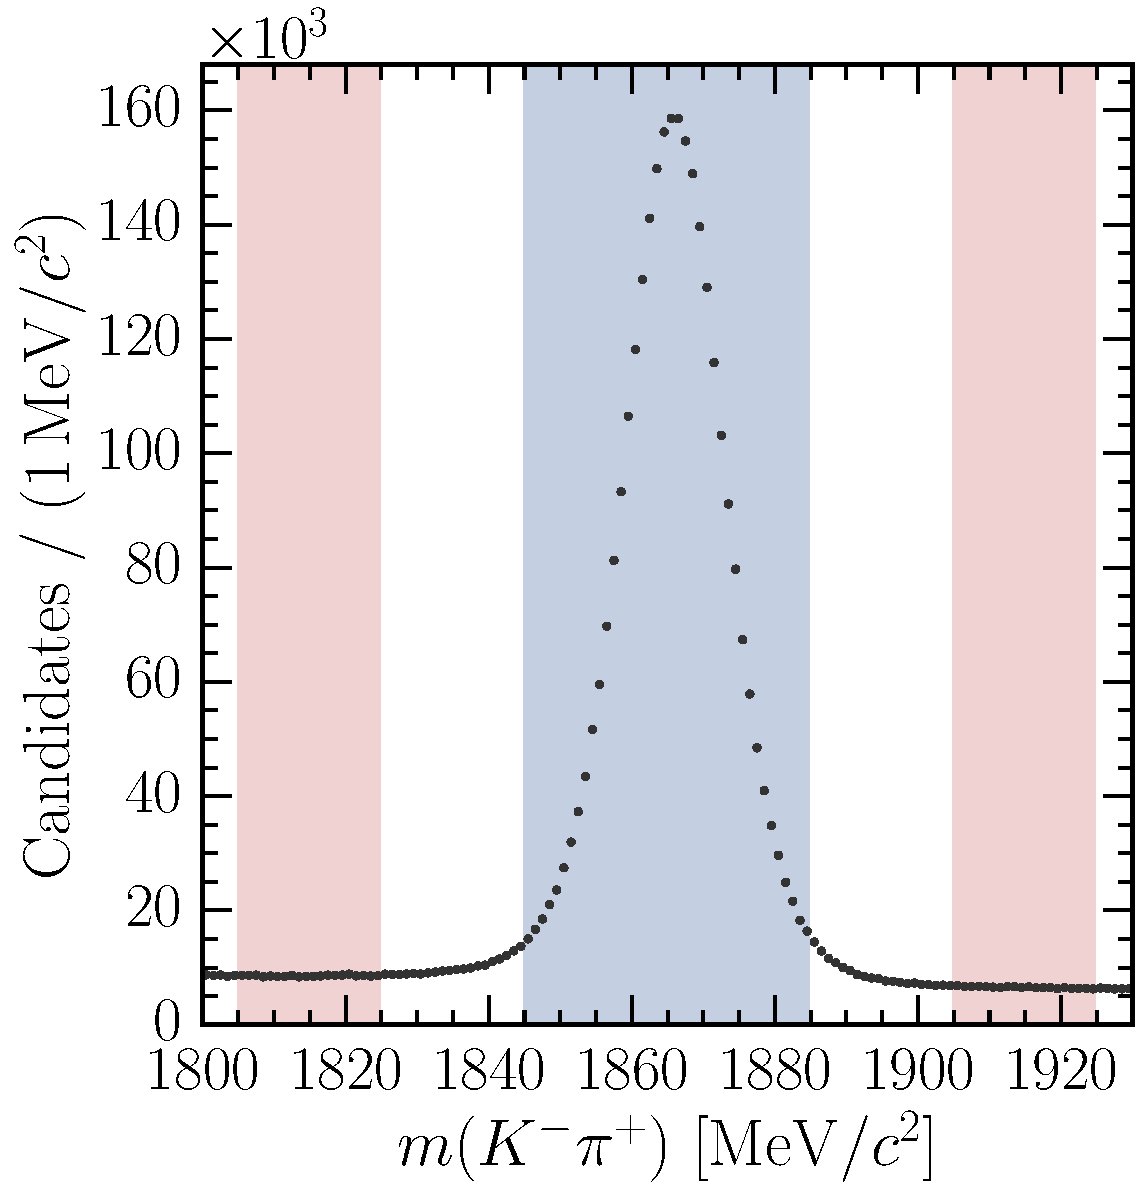
\includegraphics[width=\textwidth]{production/fitting/D0ToKpi_mass_offline_selection_regions}
    \caption{\DzToKpi}
    \label{fig:prod:fitting:regions:D0ToKpi}
  \end{subfigure}
  \begin{subfigure}{0.5\textwidth}
    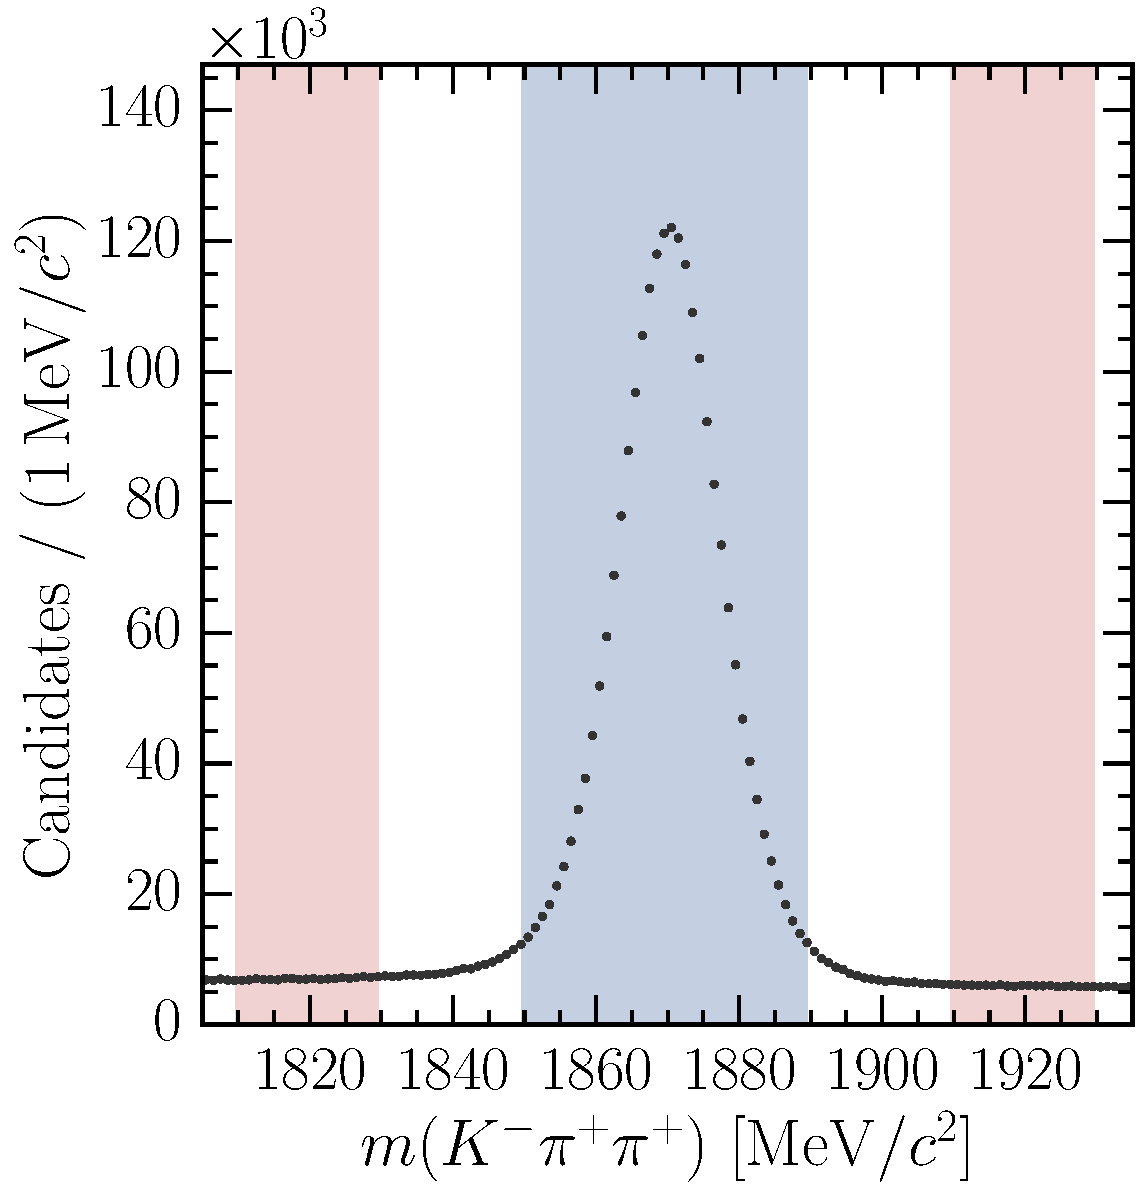
\includegraphics[width=\textwidth]{production/fitting/DpToKpipi_mass_offline_selection_regions}
    \caption{\DpToKpipi}
    \label{fig:prod:fitting:regions:DpToKpipi}
  \end{subfigure}
  \caption{%
    Definition of signal window, in blue, and sidebands, in red, for 
    \DzToKpi~(\subref*{fig:prod:fitting:regions:D0ToKpi}) and 
    \DpToKpipi~(\subref*{fig:prod:fitting:regions:DpToKpipi}) candidates.
    The boundaries of the different regions are defined in 
    \cref{chap:prod:fitting:ipchisq}.
    The full dataset is shown.
  }
  \label{fig:prod:fitting:regions_A}
\end{figure}

\begin{figure}
  \begin{subfigure}{0.5\textwidth}
    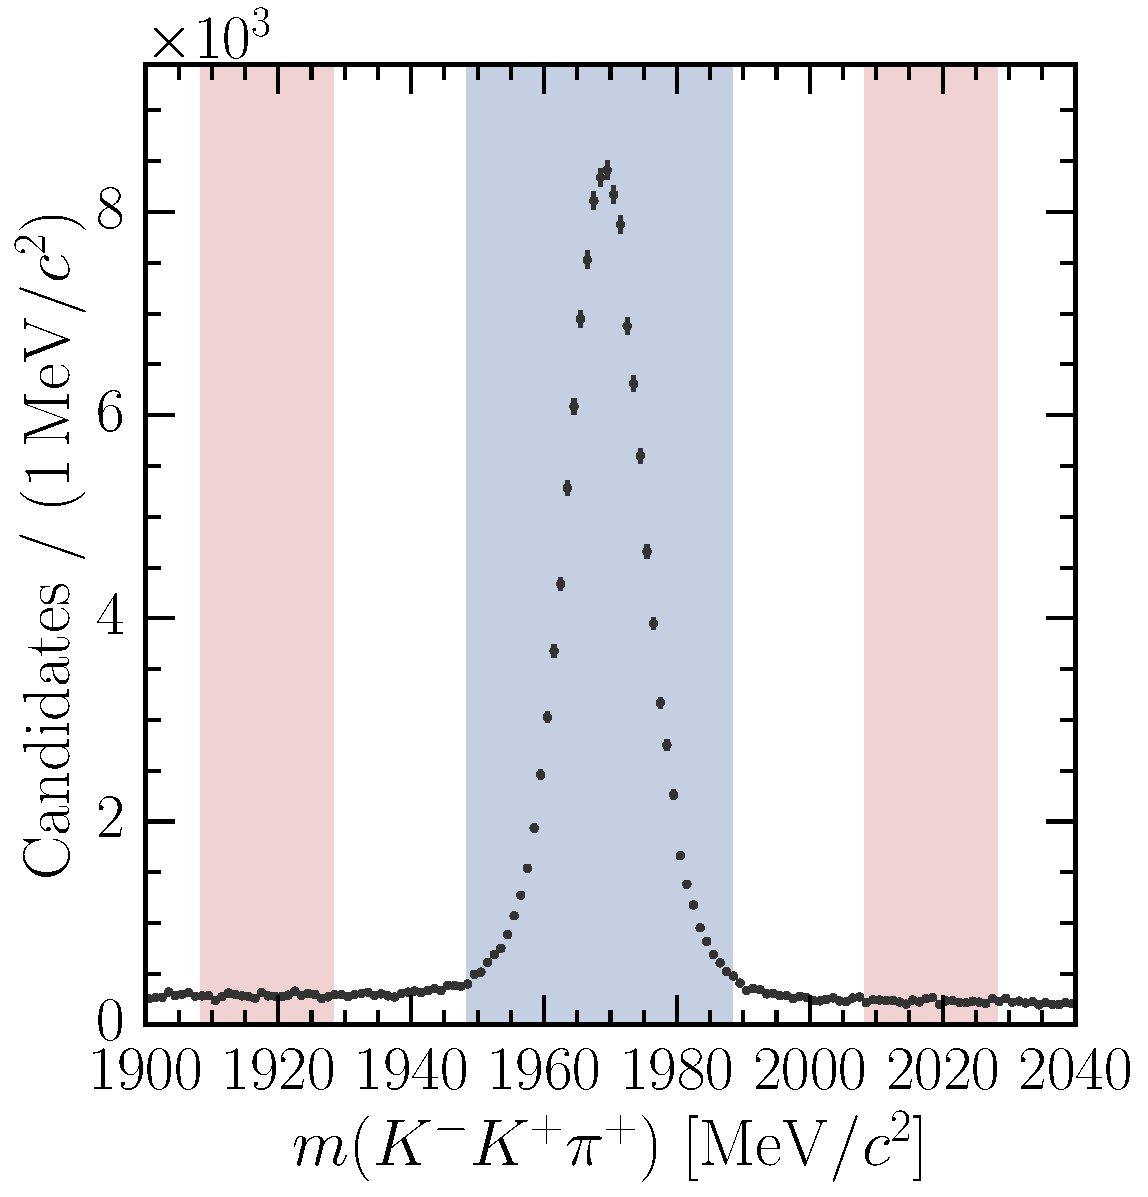
\includegraphics[width=\textwidth]{production/fitting/DsToKKpi_mass_offline_selection_regions}
    \caption{\DspTophipi}
    \label{fig:prod:fitting:regions:DsTophipi}
  \end{subfigure}
  \begin{subfigure}{0.5\textwidth}
    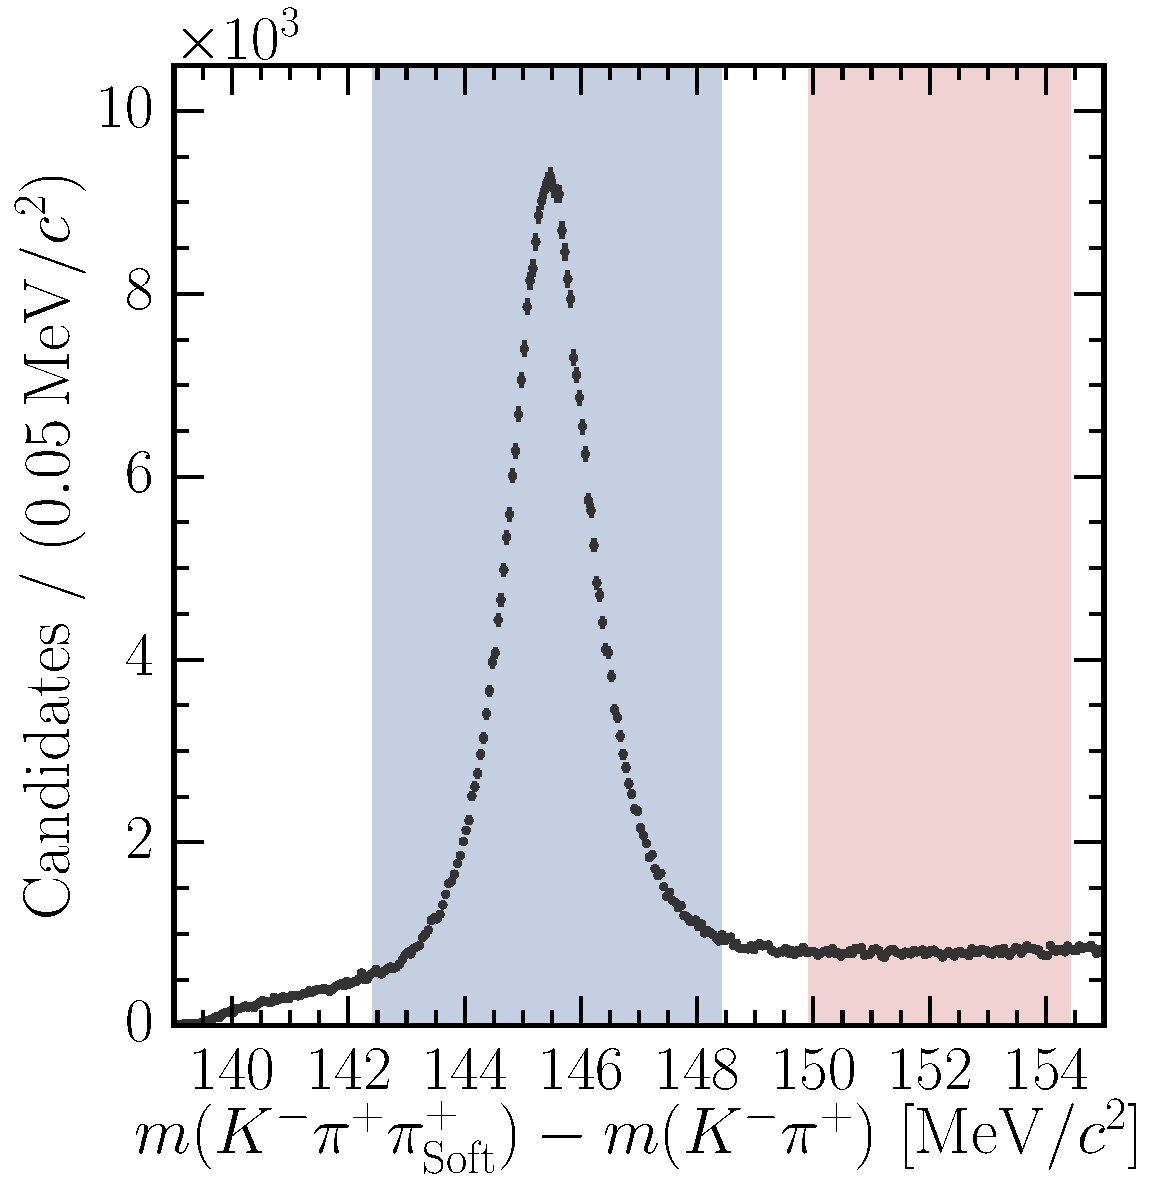
\includegraphics[width=\textwidth]{production/fitting/DstToD0pi_D0ToKpi_delta_mass_offline_selection_regions}
    \caption{\DstToDzpi}
    \label{fig:prod:fitting:regions:DstToD0pi_D0ToKpi}
  \end{subfigure}
  \caption{%
    Definition of signal window, in blue, and sidebands, in red, for 
    \DspTophipi~(\subref*{fig:prod:fitting:regions:DsTophipi}) and 
    \DstToDzpi~(\subref*{fig:prod:fitting:regions:DstToD0pi_D0ToKpi}) 
    candidates.
    The boundaries of the different regions are defined in 
    \cref{chap:prod:fitting:ipchisq}.
    The full dataset is shown.
  }
  \label{fig:prod:fitting:regions_B}
\end{figure}

\begin{figure}
  \begin{subfigure}[b]{0.5\textwidth}
    \centering
    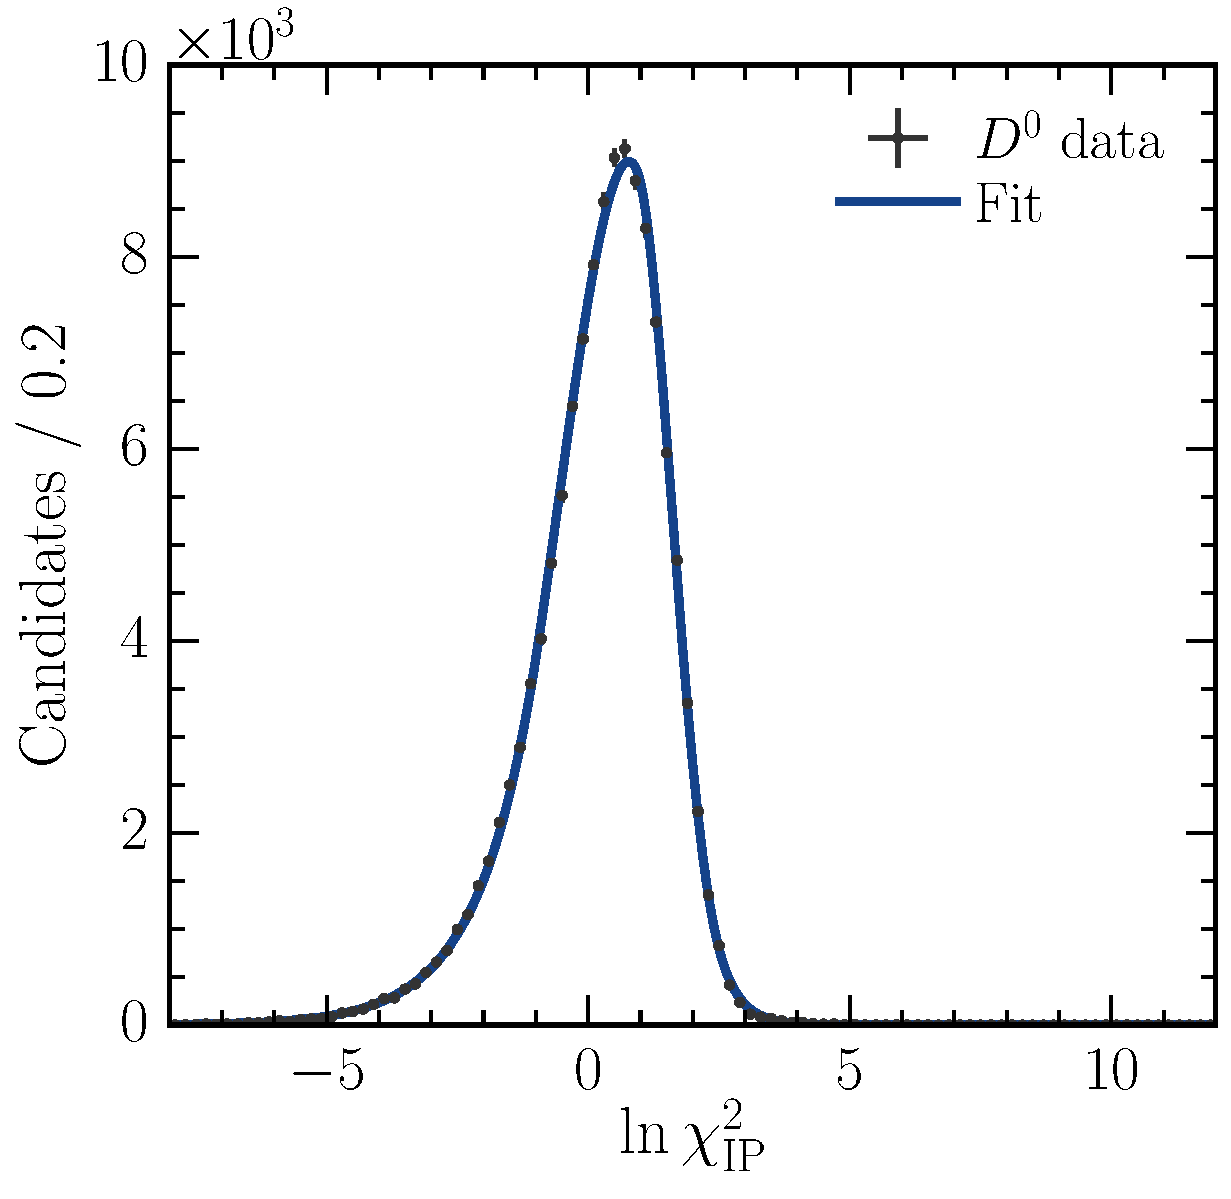
\includegraphics[width=\textwidth]{production/fitting/D0ToKpi_ipchisq_fit_pT_integrated_y_integrated_sig}
    \caption{Prompt}
    \label{fig:prod:fitting:prefits:D0ToKpi:prompt}
  \end{subfigure}
  \begin{subfigure}[b]{0.5\textwidth}
    \centering
    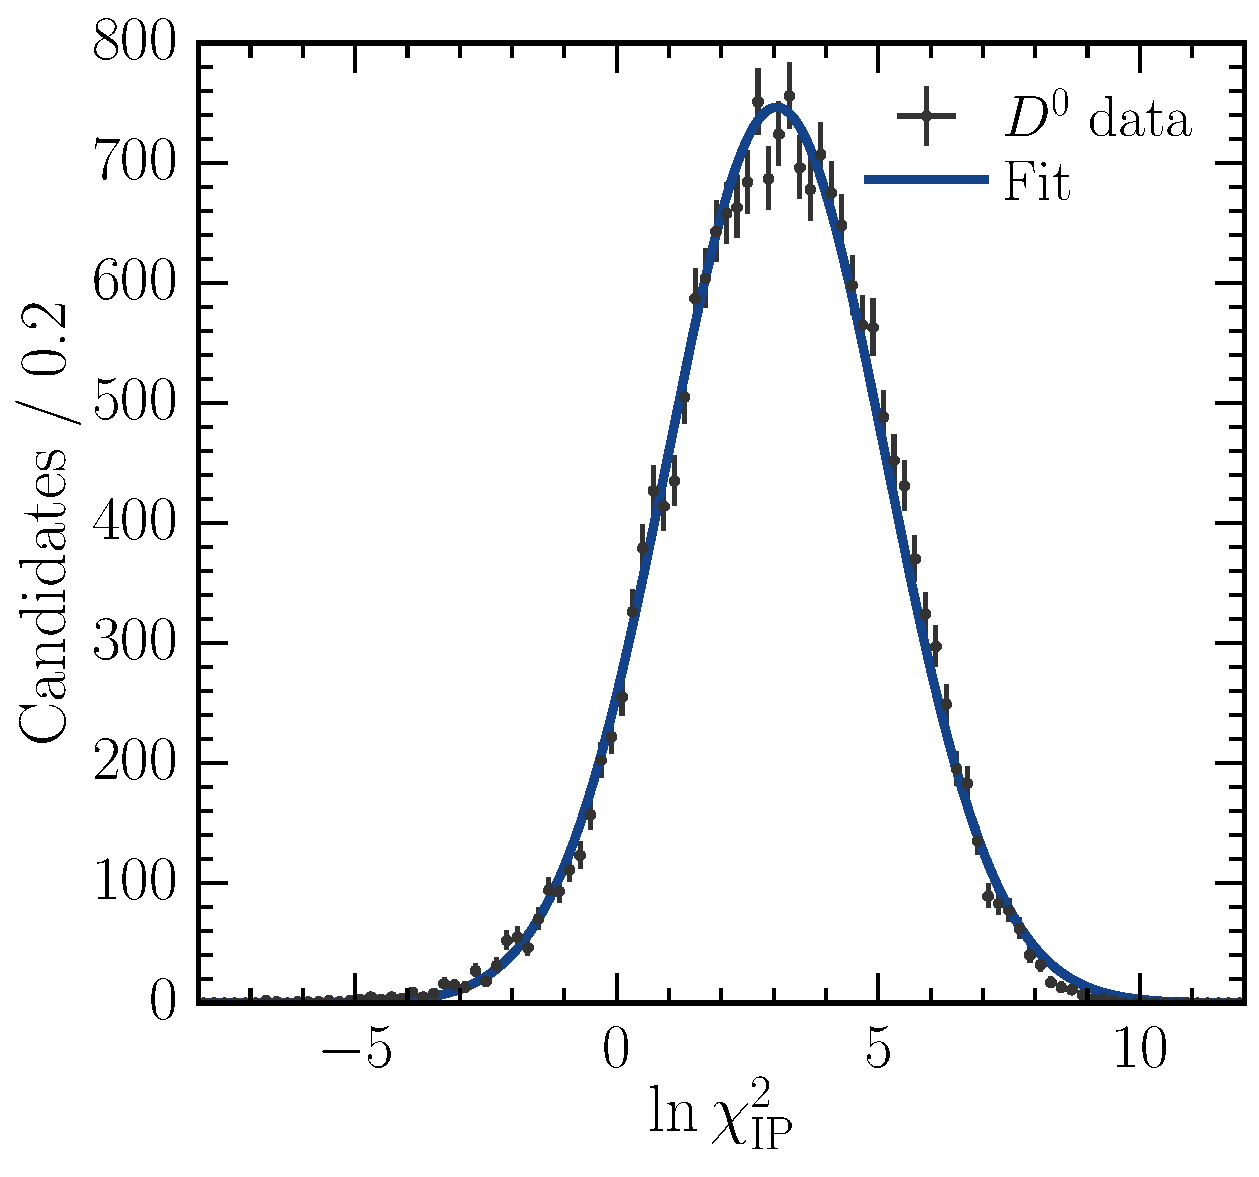
\includegraphics[width=\textwidth]{production/fitting/D0ToKpi_ipchisq_fit_pT_integrated_y_integrated_sec}
    \caption{Secondary}
    \label{fig:prod:fitting:prefits:D0ToKpi:secondary}
  \end{subfigure}
  \caption{%
    Distributions of \lnipchisq\ for simulated \DzToKpi\ decays: prompt signal 
    \PDzero (\subref*{fig:prod:fitting:prefits:D0ToKpi:prompt}) and secondary 
    signal \PDzero (\subref*{fig:prod:fitting:prefits:D0ToKpi:secondary}).
    The sum of the simultaneous likelihood fits in each \pTy\ bin is overlaid.
  }
  \label{fig:prod:fitting:prefits:D0ToKpi}
\end{figure}

\begin{figure}
  \begin{subfigure}[b]{0.5\textwidth}
    \centering
    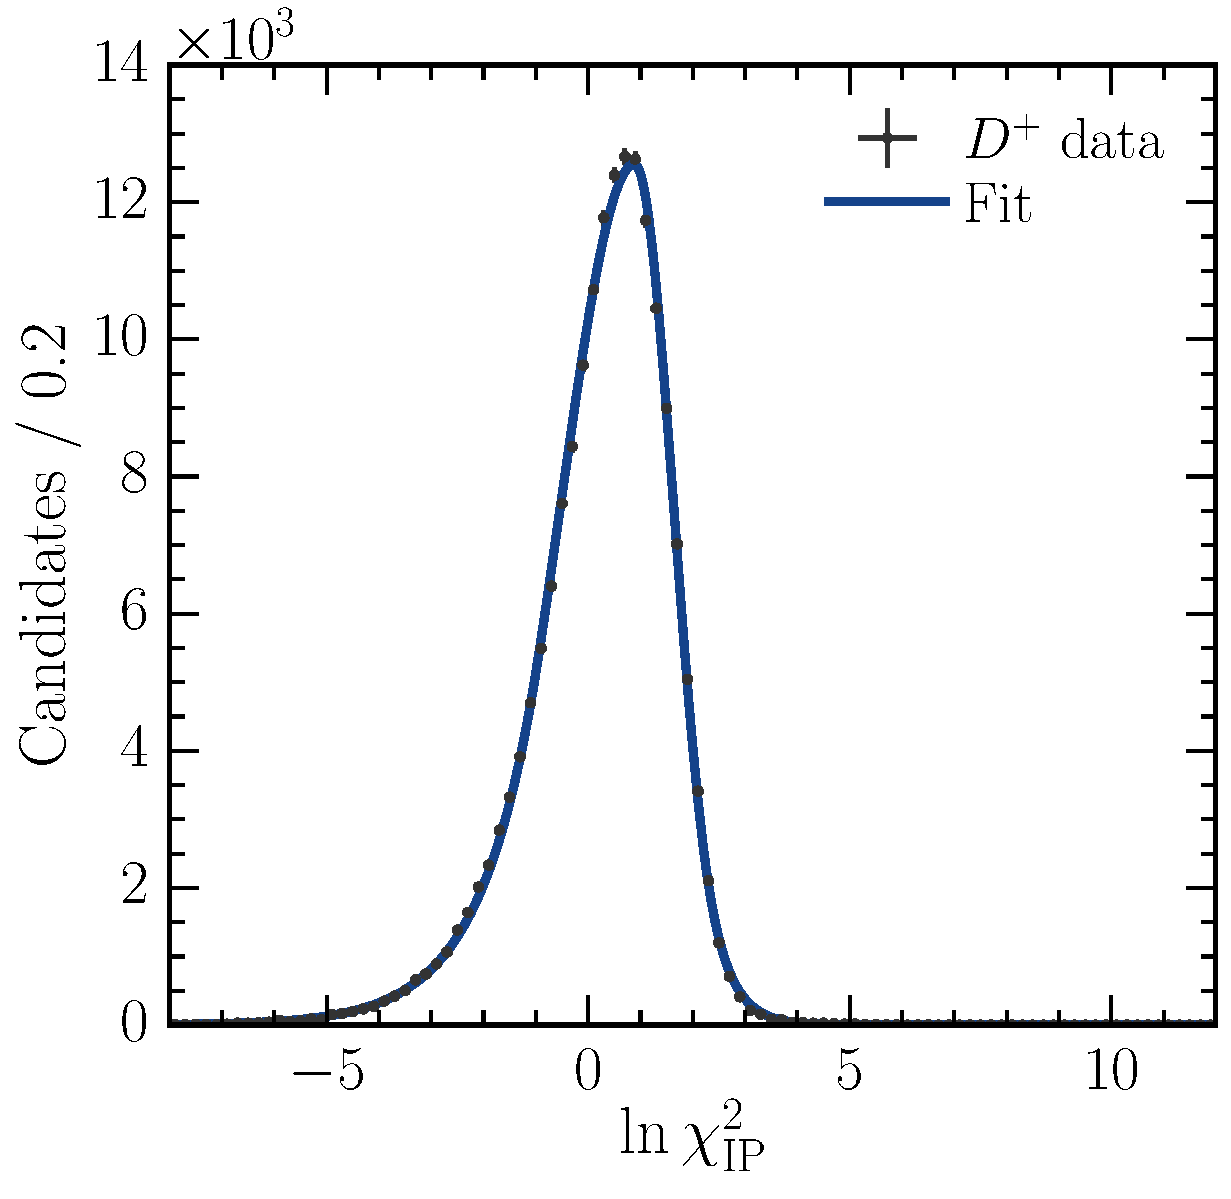
\includegraphics[width=\textwidth]{production/fitting/DpToKpipi_ipchisq_fit_pT_integrated_y_integrated_sig}
    \caption{Prompt}
    \label{fig:prod:fitting:prefits:DpToKpipi:prompt}
  \end{subfigure}
  \begin{subfigure}[b]{0.5\textwidth}
    \centering
    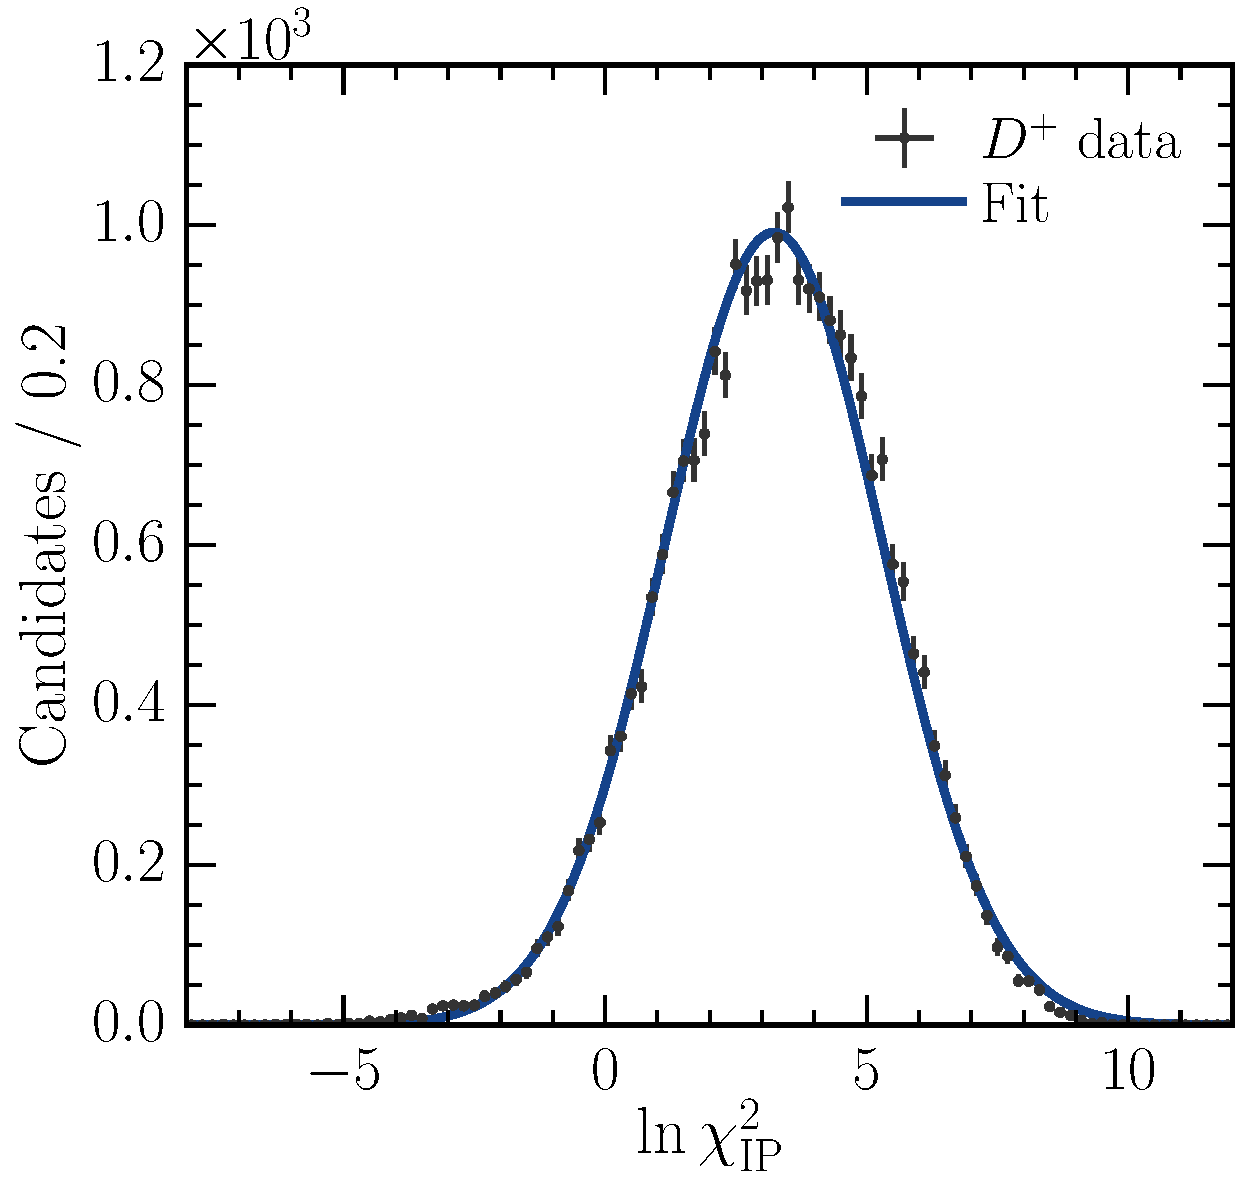
\includegraphics[width=\textwidth]{production/fitting/DpToKpipi_ipchisq_fit_pT_integrated_y_integrated_sec}
    \caption{Secondary}
    \label{fig:prod:fitting:prefits:DpToKpipi:secondary}
  \end{subfigure}
  \caption{%
    Distributions of \lnipchisq\ for simulated \DpToKpipi\ decays: prompt 
    signal \PDplus (\subref*{fig:prod:fitting:prefits:DpToKpipi:prompt}) and 
    secondary signal \PDplus 
    (\subref*{fig:prod:fitting:prefits:DpToKpipi:secondary}).
    The sum of the simultaneous likelihood fits in each \pTy\ bin is overlaid.
  }
  \label{fig:prod:fitting:prefits:DpToKpipi}
\end{figure}

\begin{figure}
  \begin{subfigure}[b]{0.5\textwidth}
    \centering
    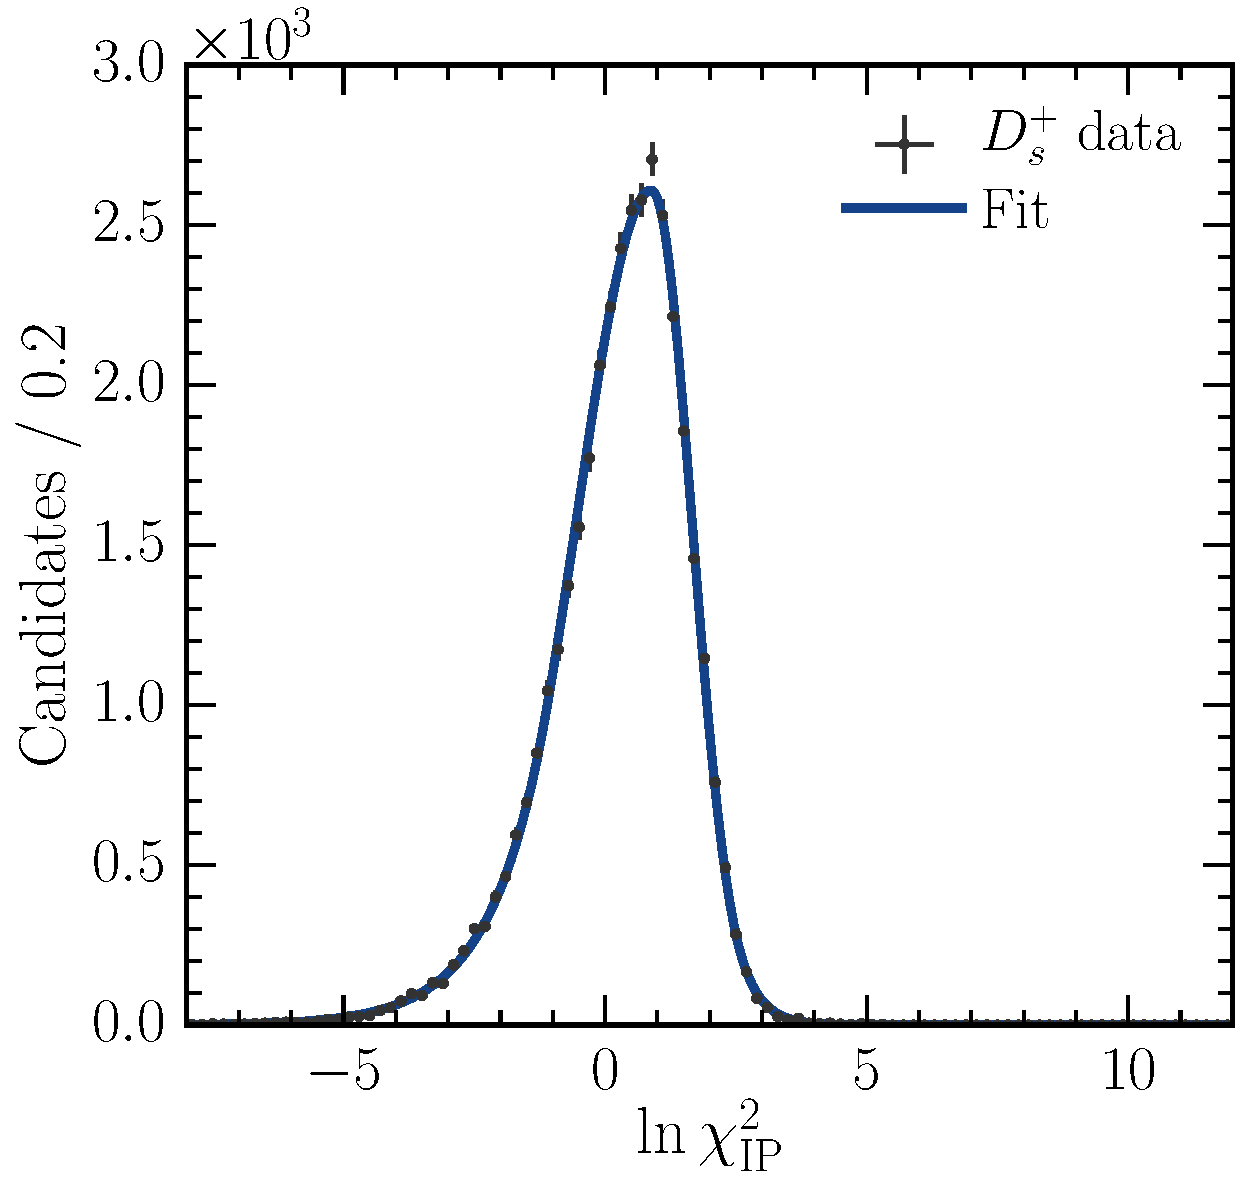
\includegraphics[width=\textwidth]{production/fitting/DsToKKpi_ipchisq_fit_pT_integrated_y_integrated_sig}
    \caption{Prompt}
    \label{fig:prod:fitting:prefits:DsToKKpi:prompt}
  \end{subfigure}
  \begin{subfigure}[b]{0.5\textwidth}
    \centering
    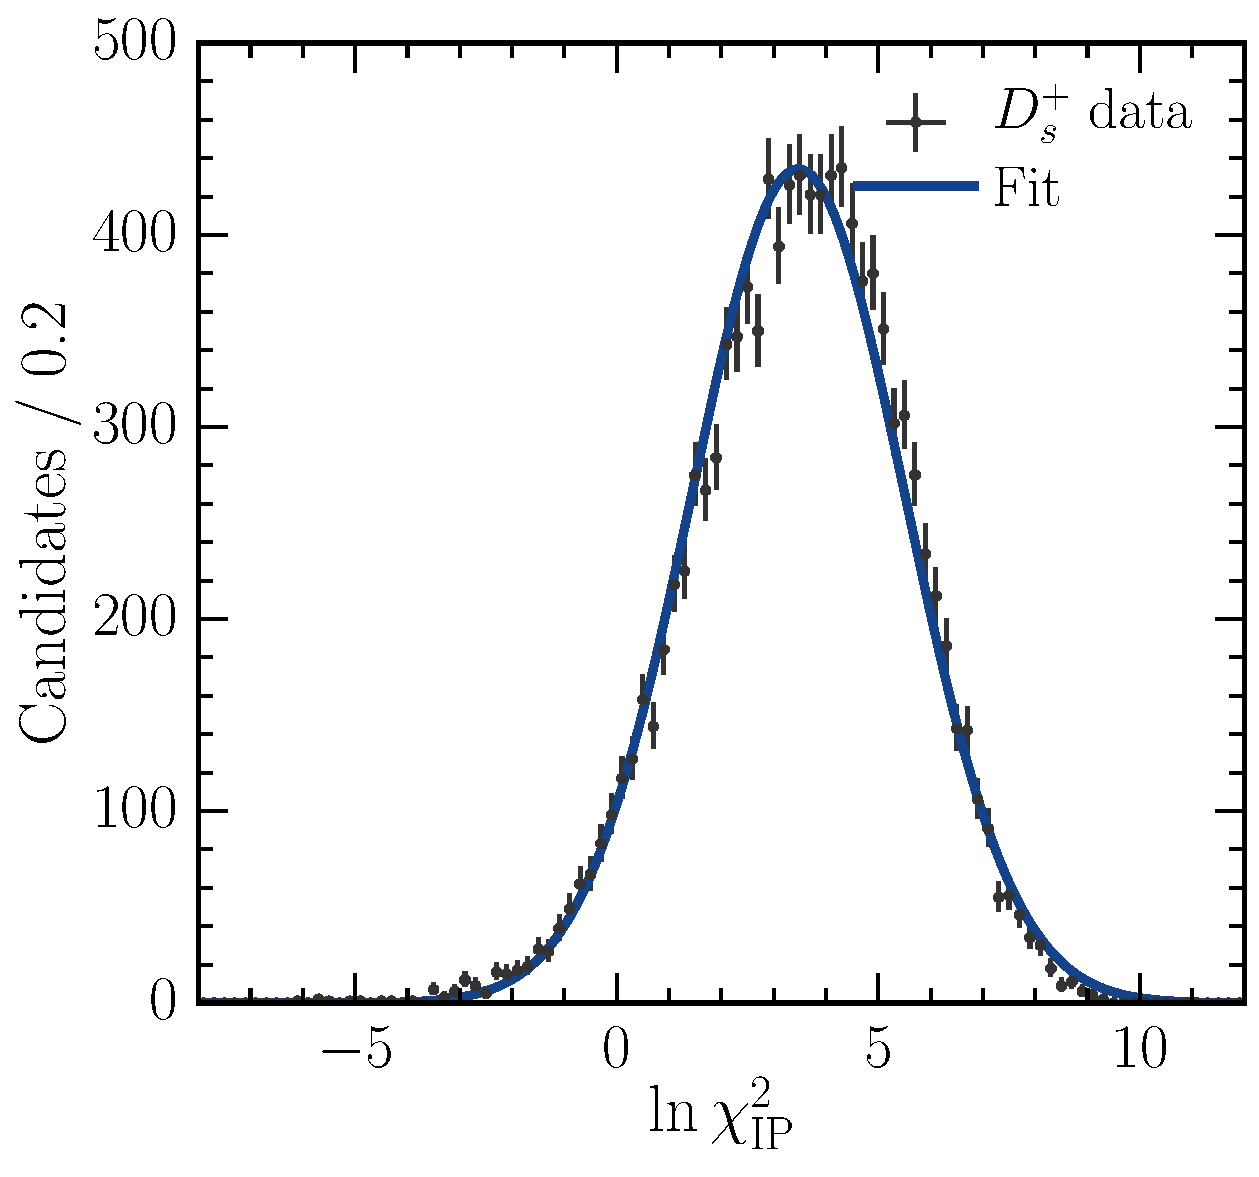
\includegraphics[width=\textwidth]{production/fitting/DsToKKpi_ipchisq_fit_pT_integrated_y_integrated_sec}
    \caption{Secondary}
    \label{fig:prod:fitting:prefits:DsToKKpi:secondary}
  \end{subfigure}
  \caption{%
    Distributions of \lnipchisq\ for simulated \DspTophipi\ decays: prompt 
    signal \PDsplus (\subref*{fig:prod:fitting:prefits:DsToKKpi:prompt}) and 
    secondary signal \PDsplus 
    (\subref*{fig:prod:fitting:prefits:DsToKKpi:secondary}).
    The sum of the simultaneous likelihood fits in each \pTy\ bin is overlaid.
  }
  \label{fig:prod:fitting:prefits:DsToKKpi}
\end{figure}

\begin{figure}
  \begin{subfigure}[b]{0.5\textwidth}
    \centering
    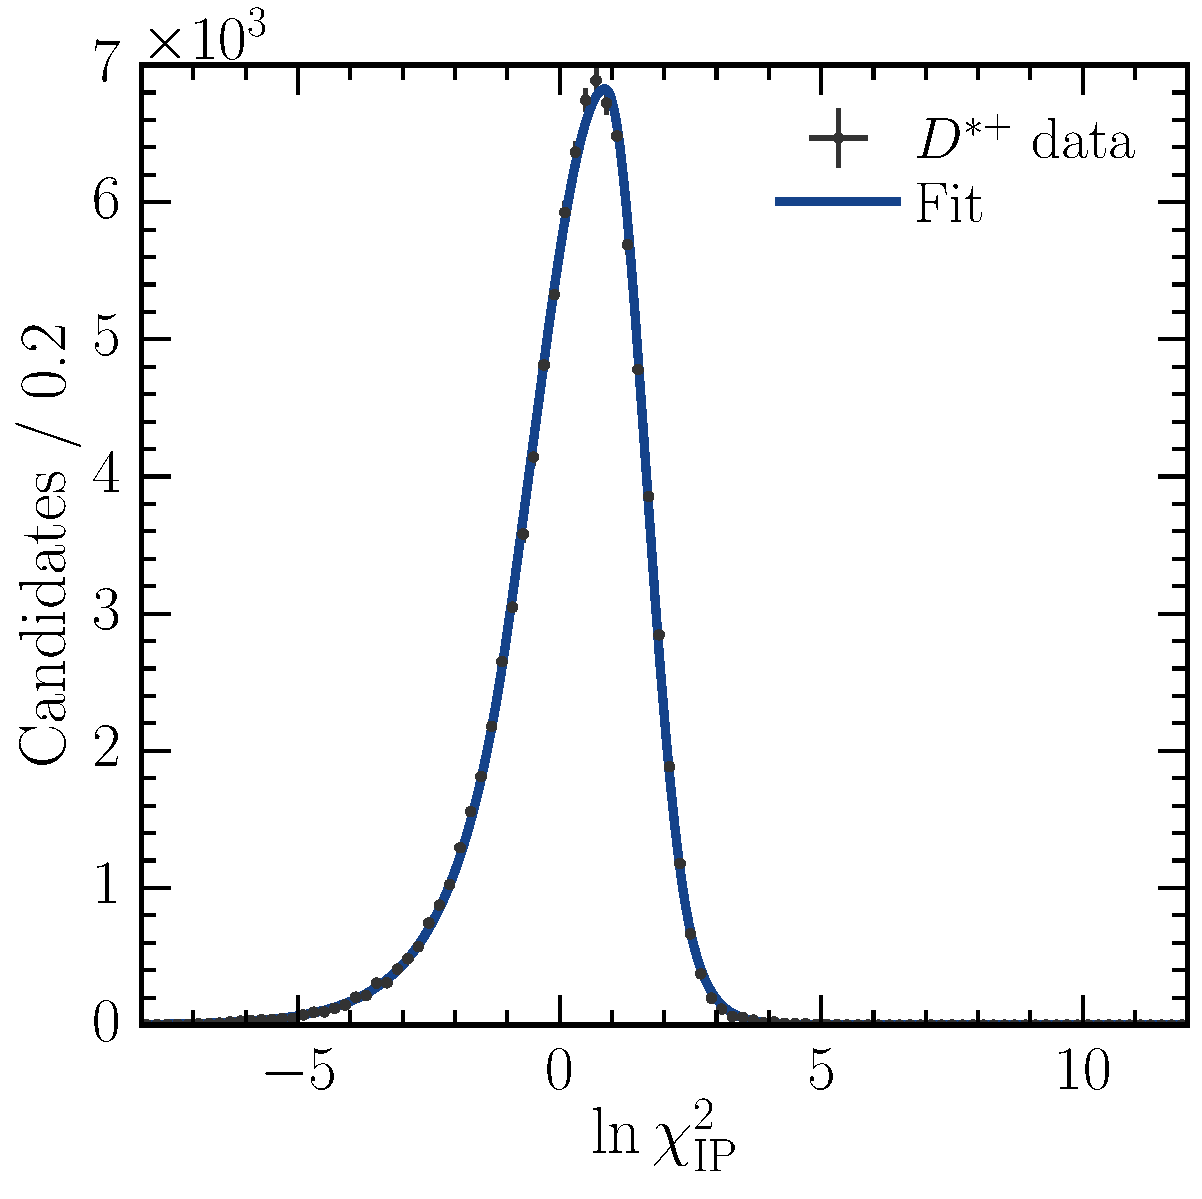
\includegraphics[width=\textwidth]{production/fitting/DstToD0pi_D0ToKpi_ipchisq_fit_pT_integrated_y_integrated_sig}
    \caption{Prompt}
    \label{fig:prod:fitting:prefits:DstToD0pi_D0ToKpi:prompt}
  \end{subfigure}
  \begin{subfigure}[b]{0.5\textwidth}
    \centering
    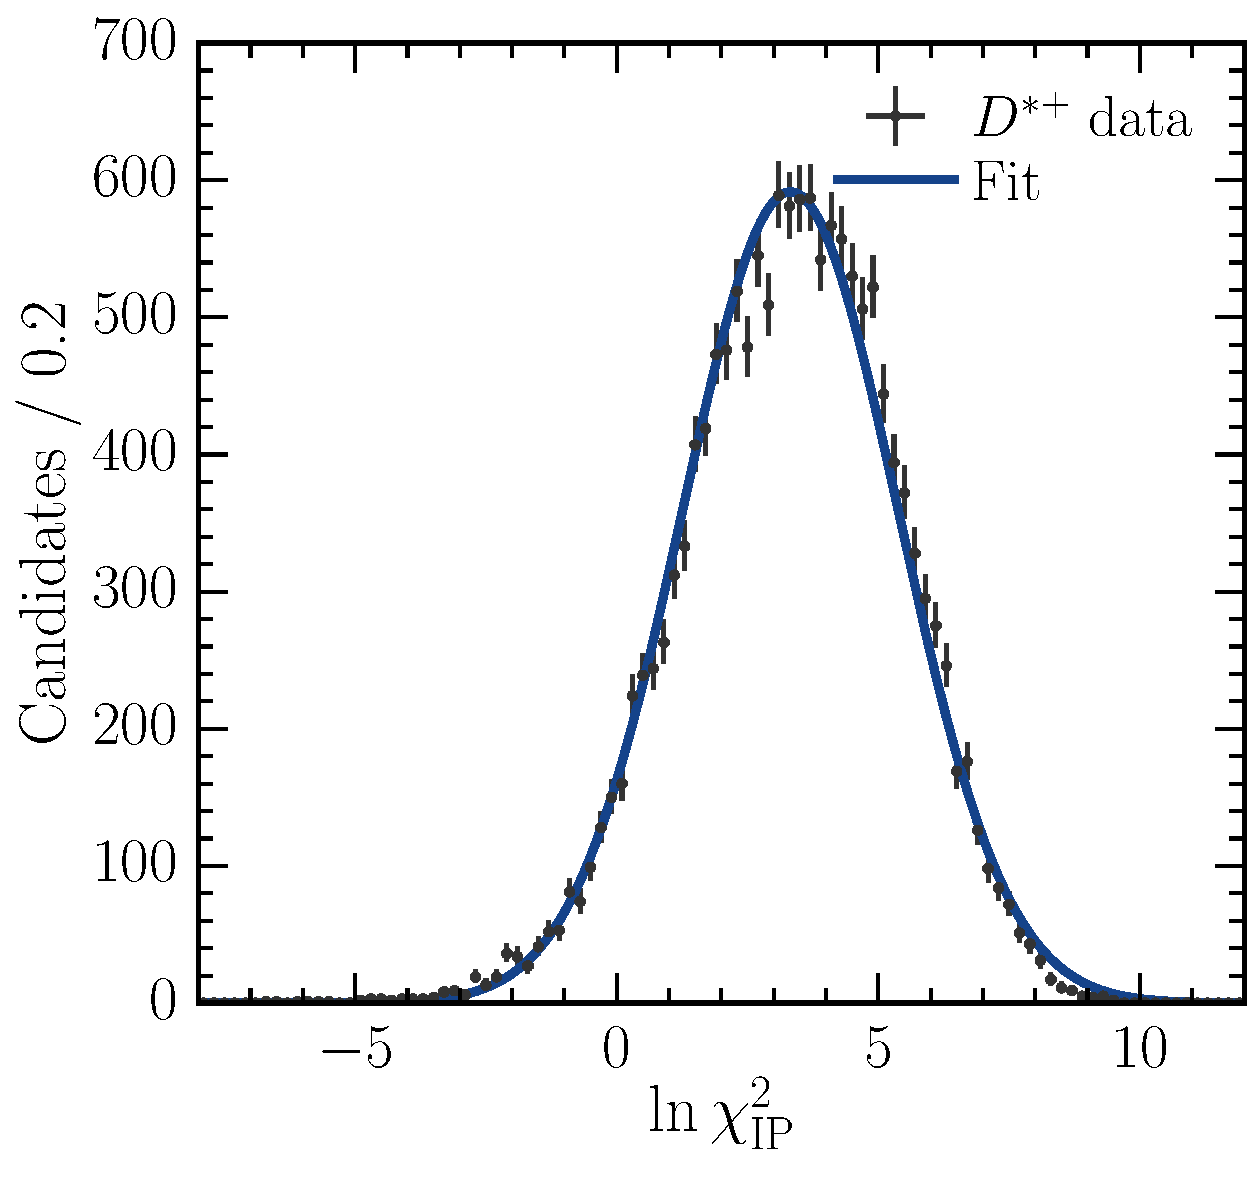
\includegraphics[width=\textwidth]{production/fitting/DstToD0pi_D0ToKpi_ipchisq_fit_pT_integrated_y_integrated_sec}
    \caption{Secondary}
    \label{fig:prod:fitting:prefits:DstToD0pi_D0ToKpi:secondary}
  \end{subfigure}
  \caption{%
    Distributions of \PDzero \lnipchisq\ for simulated \DstToDzpi, with 
    \DzToKpi, decays: prompt signal \PDstarp\
    (\subref*{fig:prod:fitting:prefits:DstToD0pi_D0ToKpi:prompt}) and secondary 
    signal \PDstarp\
    (\subref*{fig:prod:fitting:prefits:DstToD0pi_D0ToKpi:secondary}).
    The sum of the simultaneous likelihood fits in each \pTy\ bin is overlaid.
  }
  \label{fig:prod:fitting:prefits:DstToD0pi_D0ToKpi}
\end{figure}

\begin{figure}
  \begin{subfigure}[b]{0.5\textwidth}
    \centering
    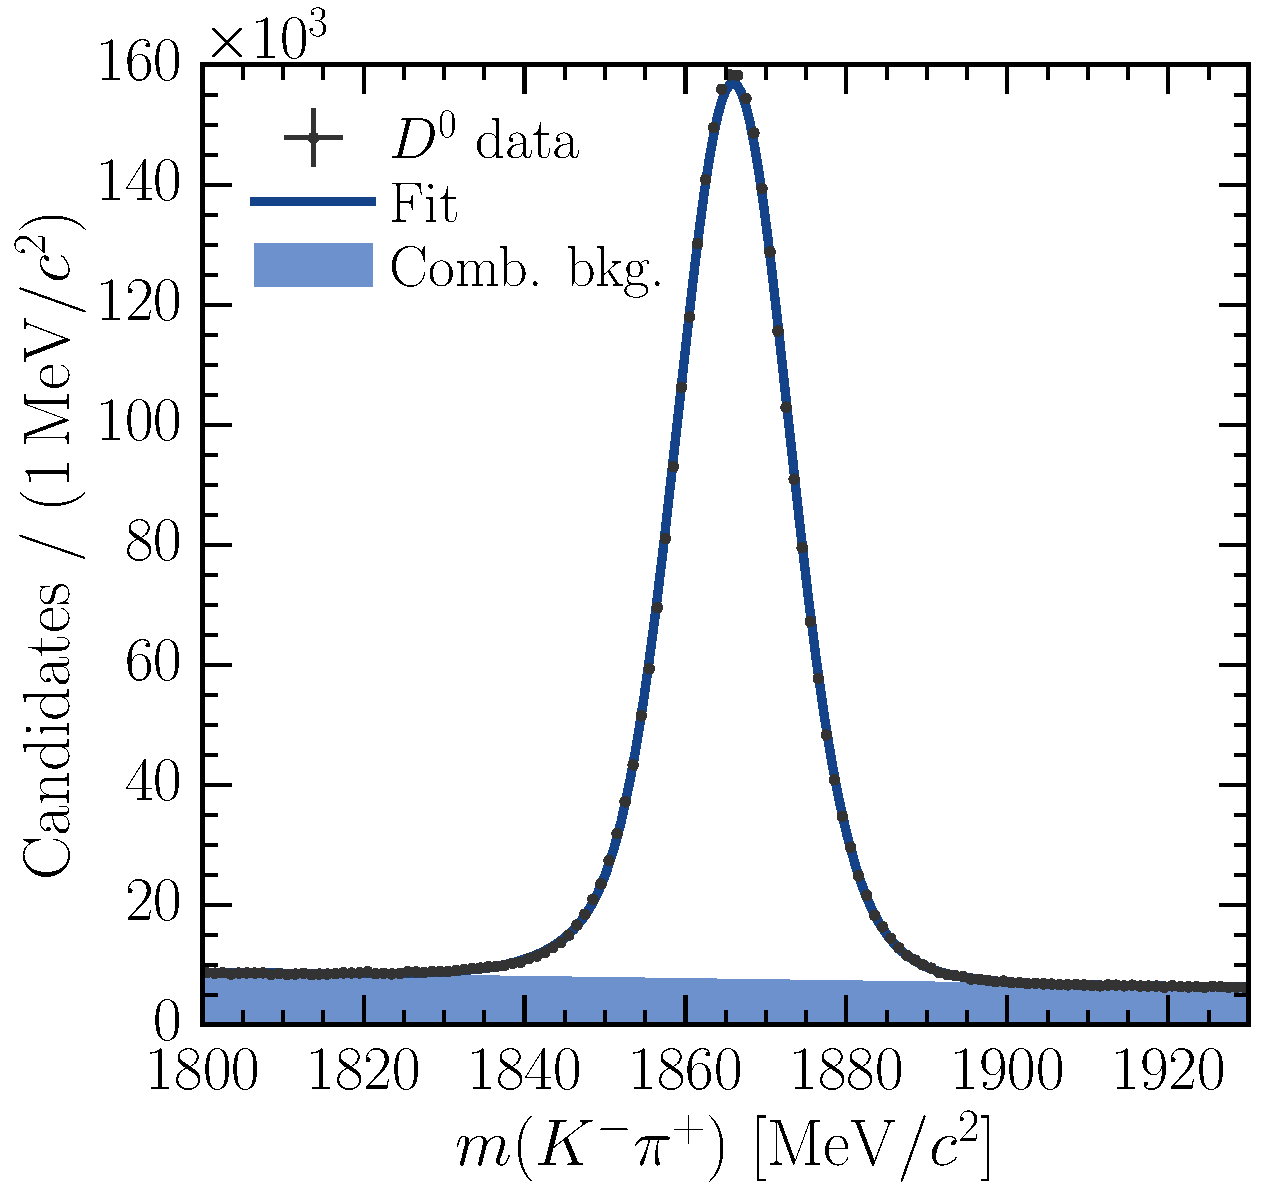
\includegraphics[width=\textwidth]{production/fitting/D0ToKpi_mass_fit_pT_integrated_y_integrated}
    \caption{Mass}
    \label{fig:prod:fitting:D0ToKpi:mass}
  \end{subfigure}
  \begin{subfigure}[b]{0.5\textwidth}
    \centering
    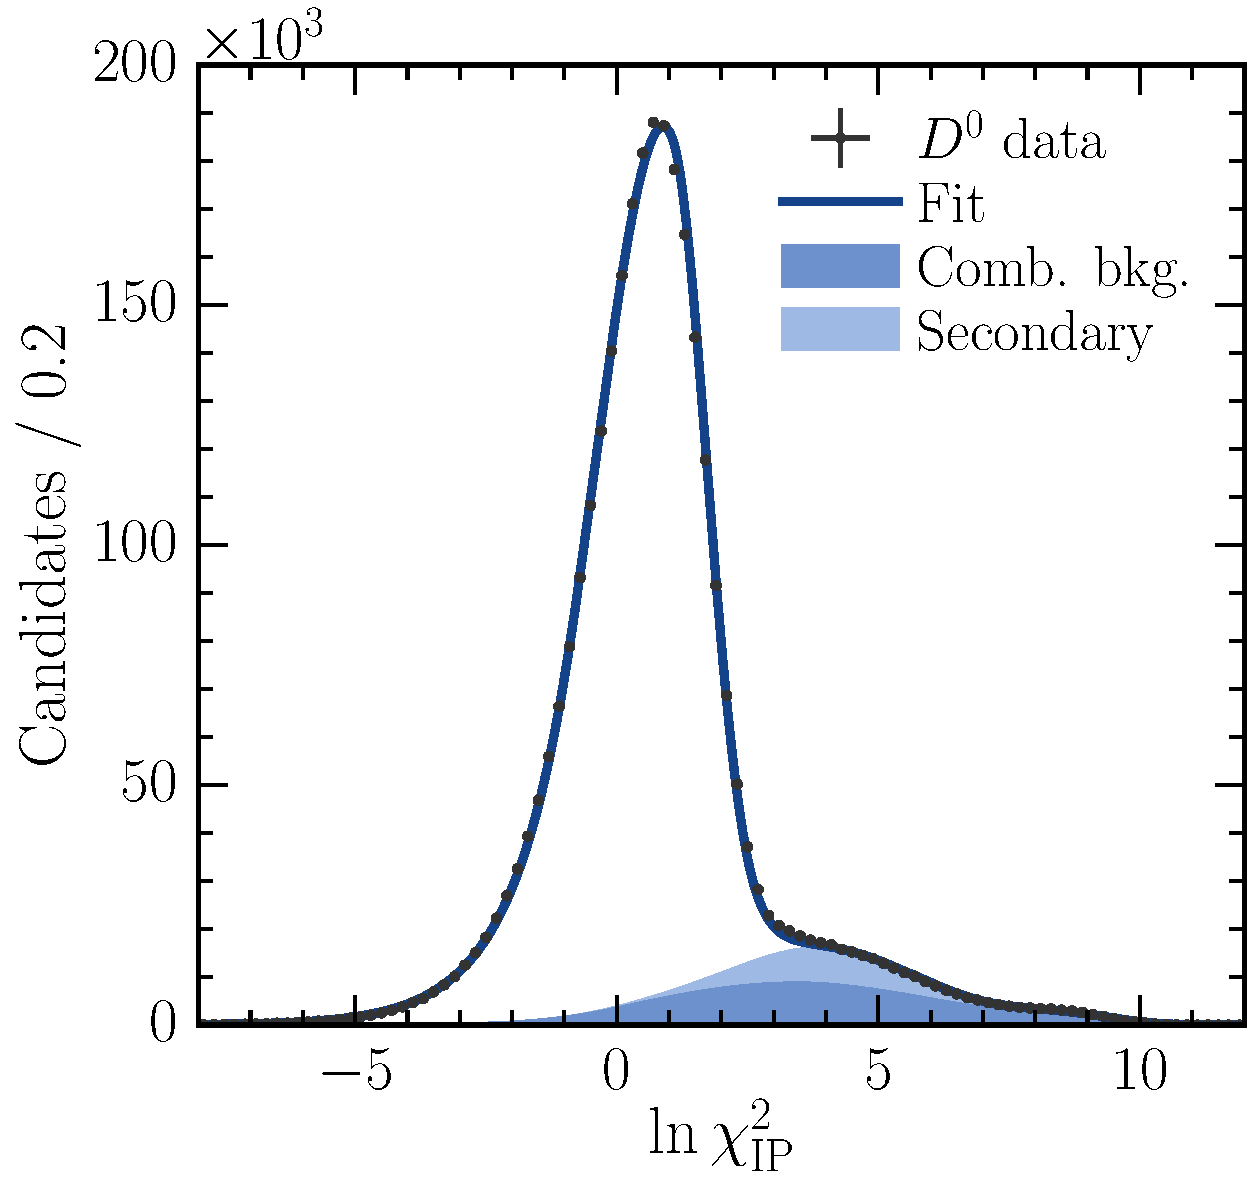
\includegraphics[width=\textwidth]{production/fitting/D0ToKpi_ipchisq_fit_pT_integrated_y_integrated}
    \caption{\lnipchisq}
    \label{fig:prod:fitting:D0ToKpi:ipchisq}
  \end{subfigure}
  \caption{%
    Distributions for fully selected \DzToKpi\ candidates: \PDzero\ invariant 
    mass (\subref*{fig:prod:fitting:D0ToKpi:mass}) and \PDzero\ \lnipchisq\ 
    (\subref*{fig:prod:fitting:D0ToKpi:ipchisq}) for a mass window of 
    $\pm\SI{20}{\MeVcc}$ around the nominal \PDzero mass.
    The sum of the simultaneous likelihood fits in each \pTy\ bin is shown, 
    with components as indicated in the legends.
  }
  \label{fig:prod:fitting:D0ToKpi}
\end{figure}

\begin{figure}
  \begin{subfigure}[b]{0.5\textwidth}
    \centering
    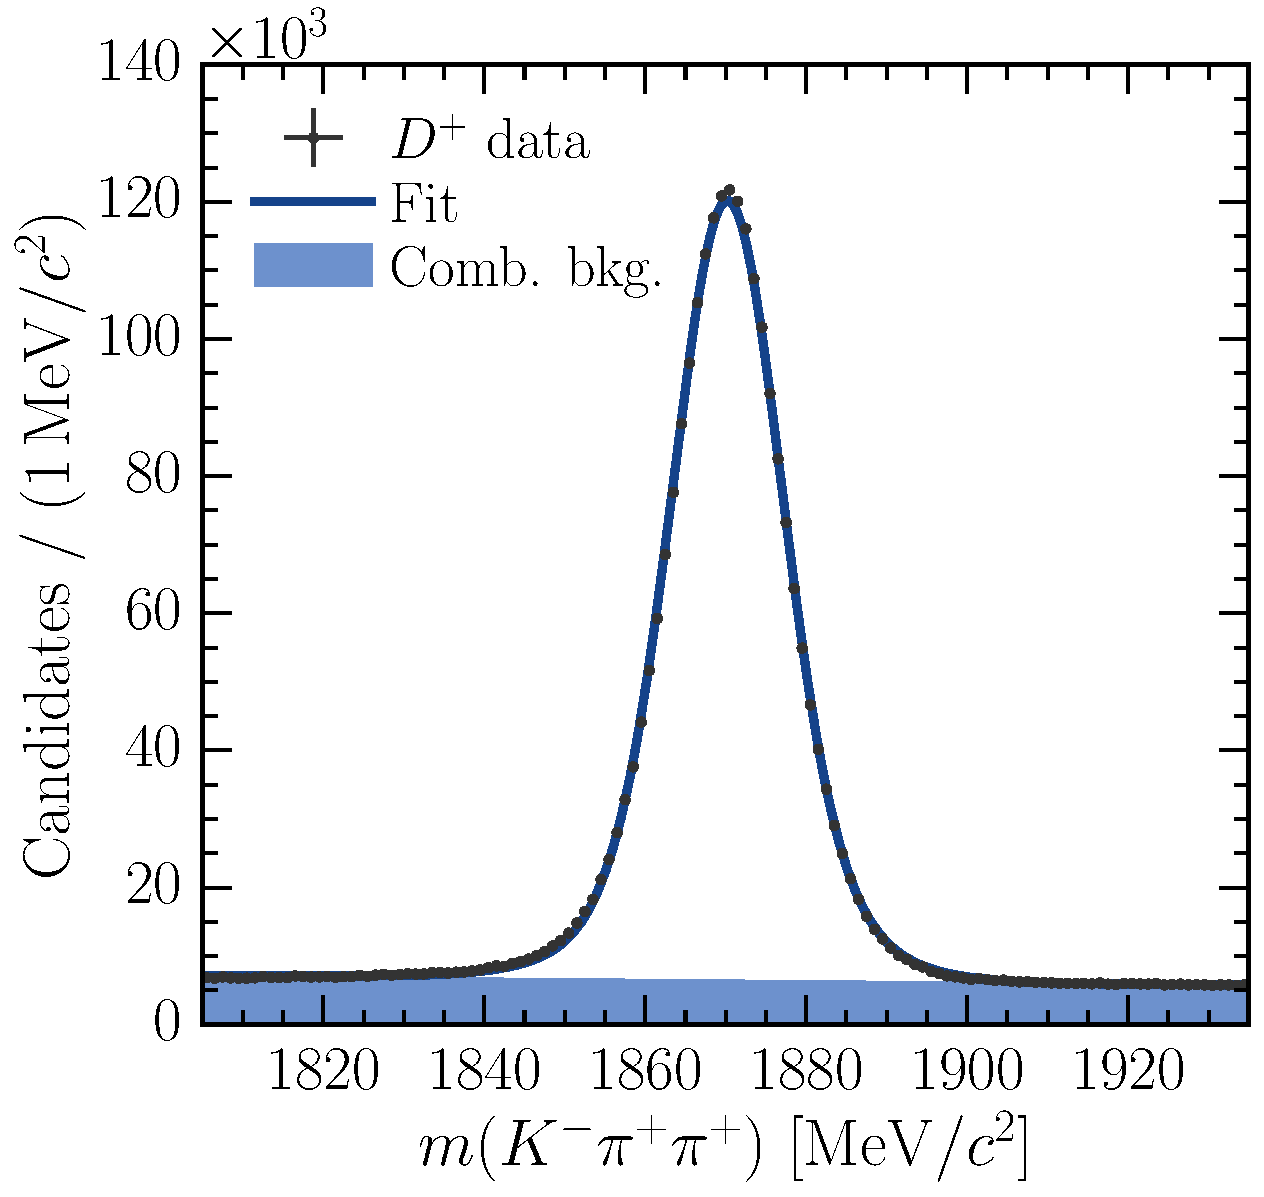
\includegraphics[width=\textwidth]{production/fitting/DpToKpipi_mass_fit_pT_integrated_y_integrated}
    \caption{Mass}
    \label{fig:prod:fitting:DpToKpipi:mass}
  \end{subfigure}
  \begin{subfigure}[b]{0.5\textwidth}
    \centering
    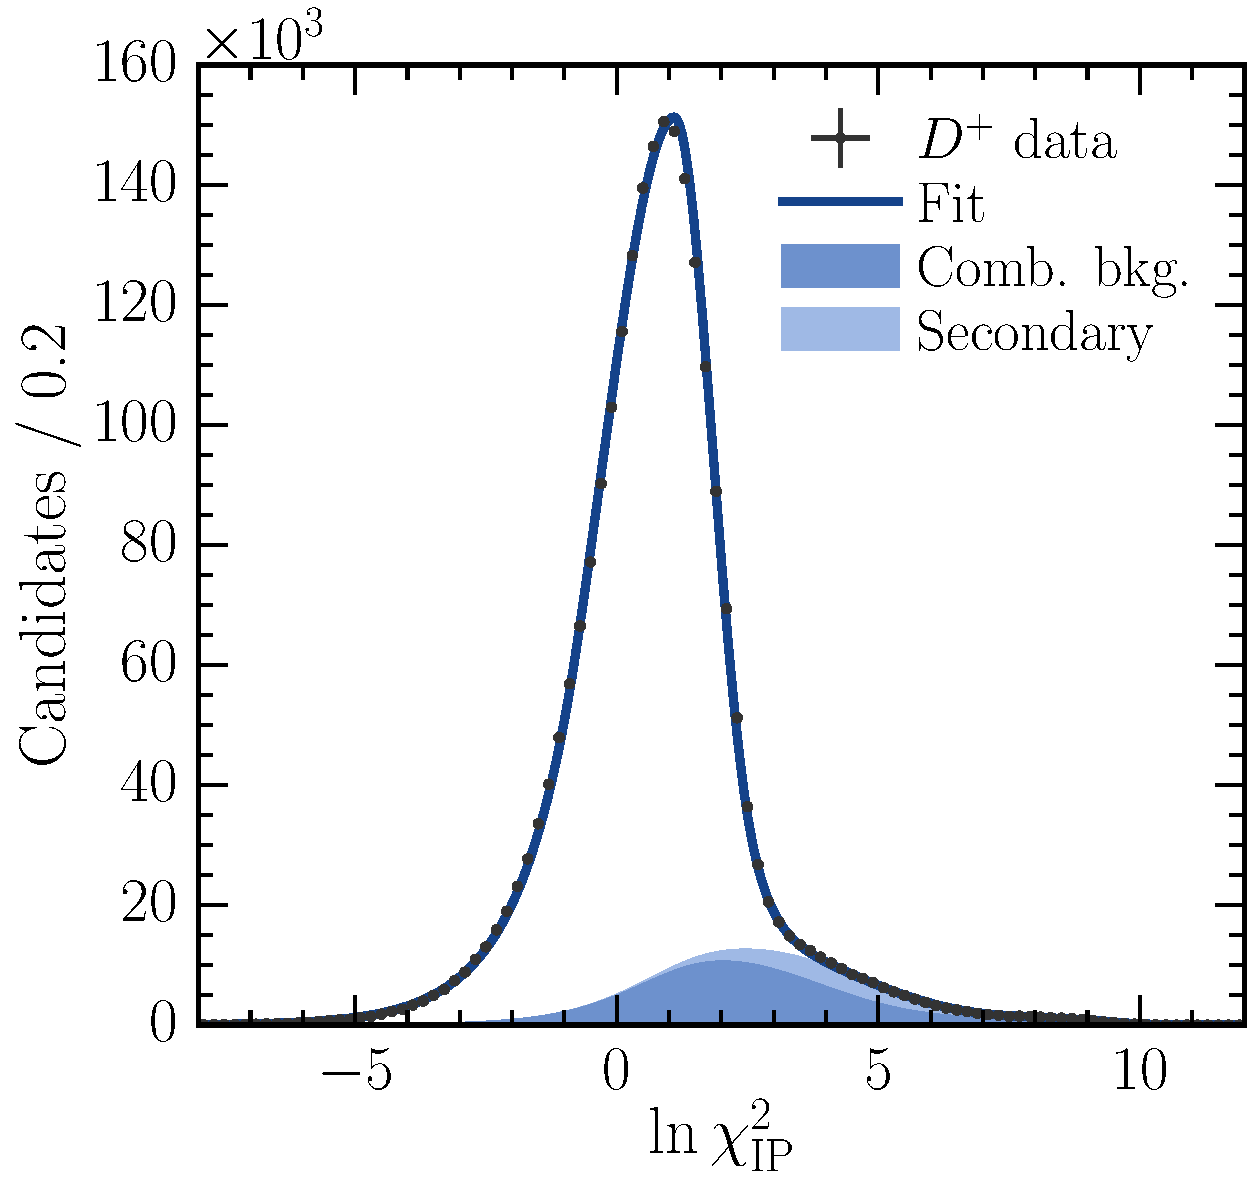
\includegraphics[width=\textwidth]{production/fitting/DpToKpipi_ipchisq_fit_pT_integrated_y_integrated}
    \caption{\lnipchisq}
    \label{fig:prod:fitting:DpToKpipi:ipchisq}
  \end{subfigure}
  \caption{%
    Distributions for fully selected \DpToKpipi\ candidates: \PDplus\ invariant 
    mass (\subref*{fig:prod:fitting:DpToKpipi:mass}) and \PDplus\ \lnipchisq\ 
    (\subref*{fig:prod:fitting:DpToKpipi:ipchisq}) for a mass window of 
    $\pm\SI{20}{\MeVcc}$ around the nominal \PDplus mass.
    The sum of the simultaneous likelihood fits in each \pTy\ bin is shown, 
    with components as indicated in the legends.
  }
  \label{fig:prod:fitting:DpToKpipi}
\end{figure}

\begin{figure}
  \begin{subfigure}[b]{0.5\textwidth}
    \centering
    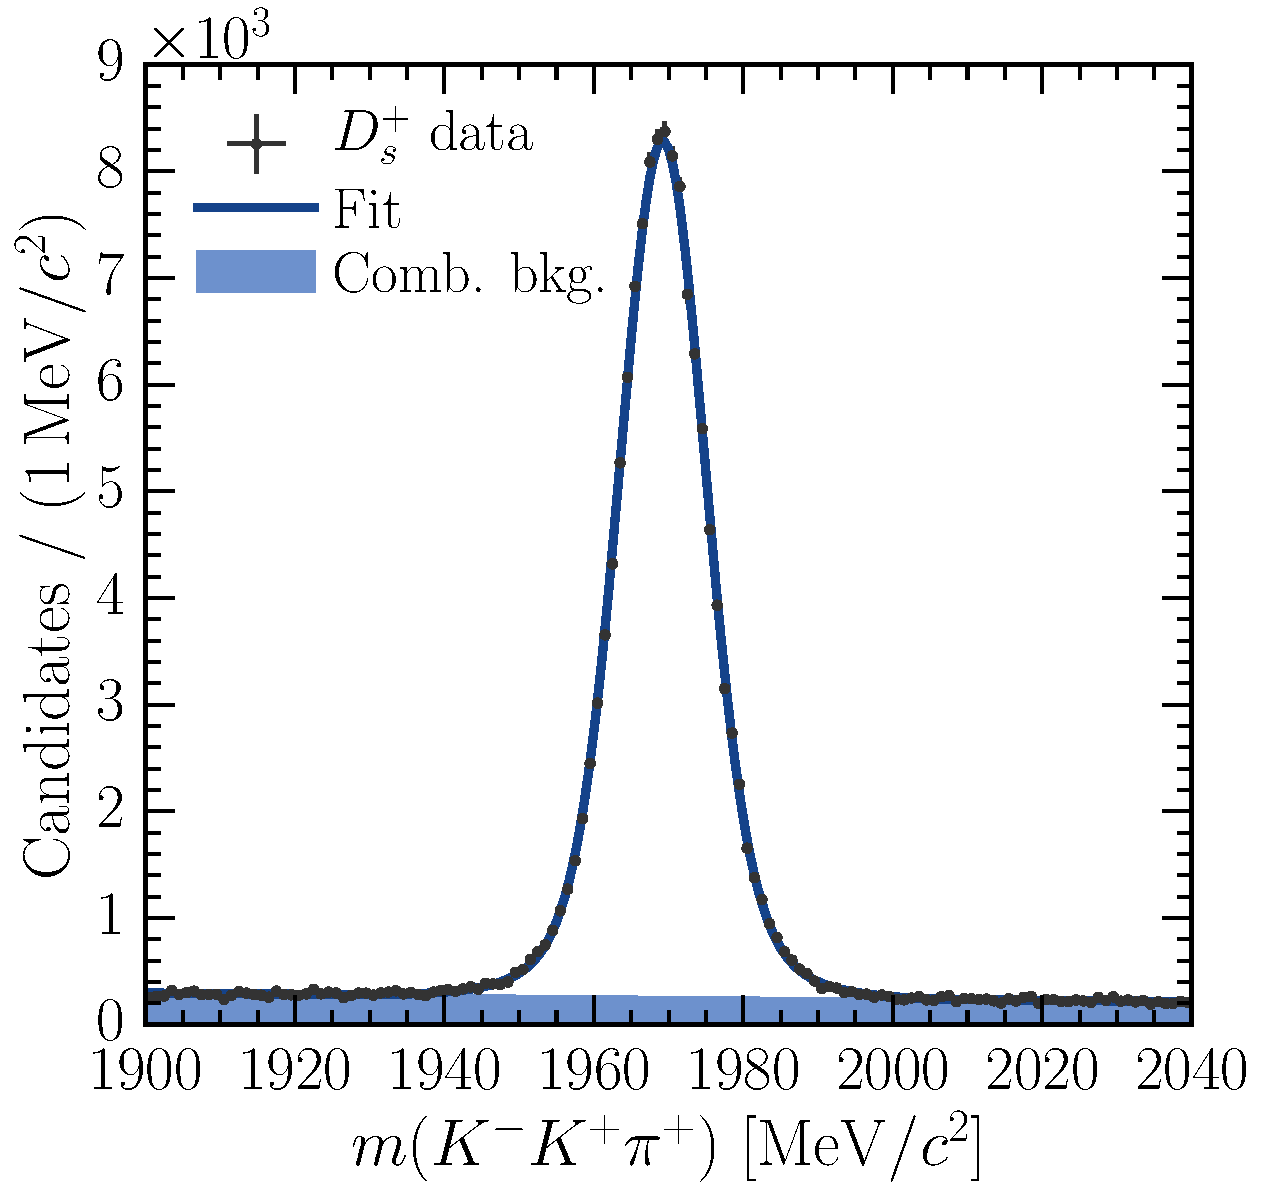
\includegraphics[width=\textwidth]{production/fitting/DsToKKpi_mass_fit_pT_integrated_y_integrated}
    \caption{Mass}
    \label{fig:prod:fitting:DsToKKpi:mass}
  \end{subfigure}
  \begin{subfigure}[b]{0.5\textwidth}
    \centering
    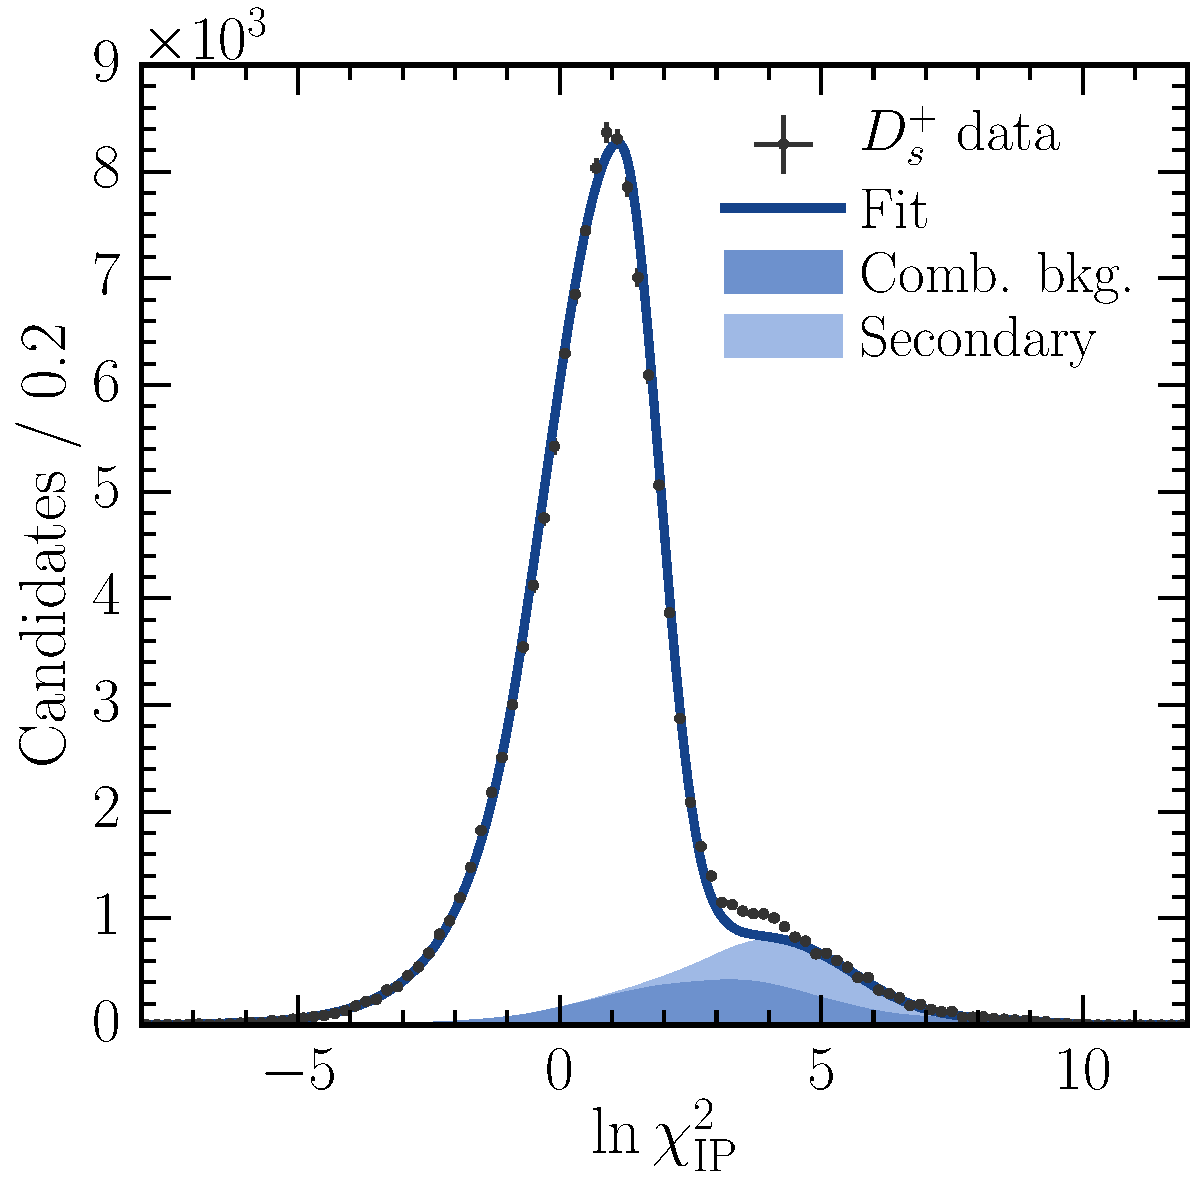
\includegraphics[width=\textwidth]{production/fitting/DsToKKpi_ipchisq_fit_pT_integrated_y_integrated}
    \caption{\lnipchisq}
    \label{fig:prod:fitting:DsToKKpi:ipchisq}
  \end{subfigure}
  \caption{%
    Distributions for fully selected \DspTophipi\ candidates: \PDsplus\ 
    invariant mass (\subref*{fig:prod:fitting:DpToKpipi:mass}) and \PDsplus\ 
    \lnipchisq\ (\subref*{fig:prod:fitting:DpToKpipi:ipchisq}) for a mass 
    window of $\pm\SI{20}{\MeVcc}$ around the nominal \PDsplus mass.
    The sum of the simultaneous likelihood fits in each \pTy\ bin is shown, 
    with components as indicated in the legends.
  }
  \label{fig:prod:fitting:DsToKKpi}
\end{figure}

\begin{figure}
  \begin{subfigure}[b]{0.5\textwidth}
    \centering
    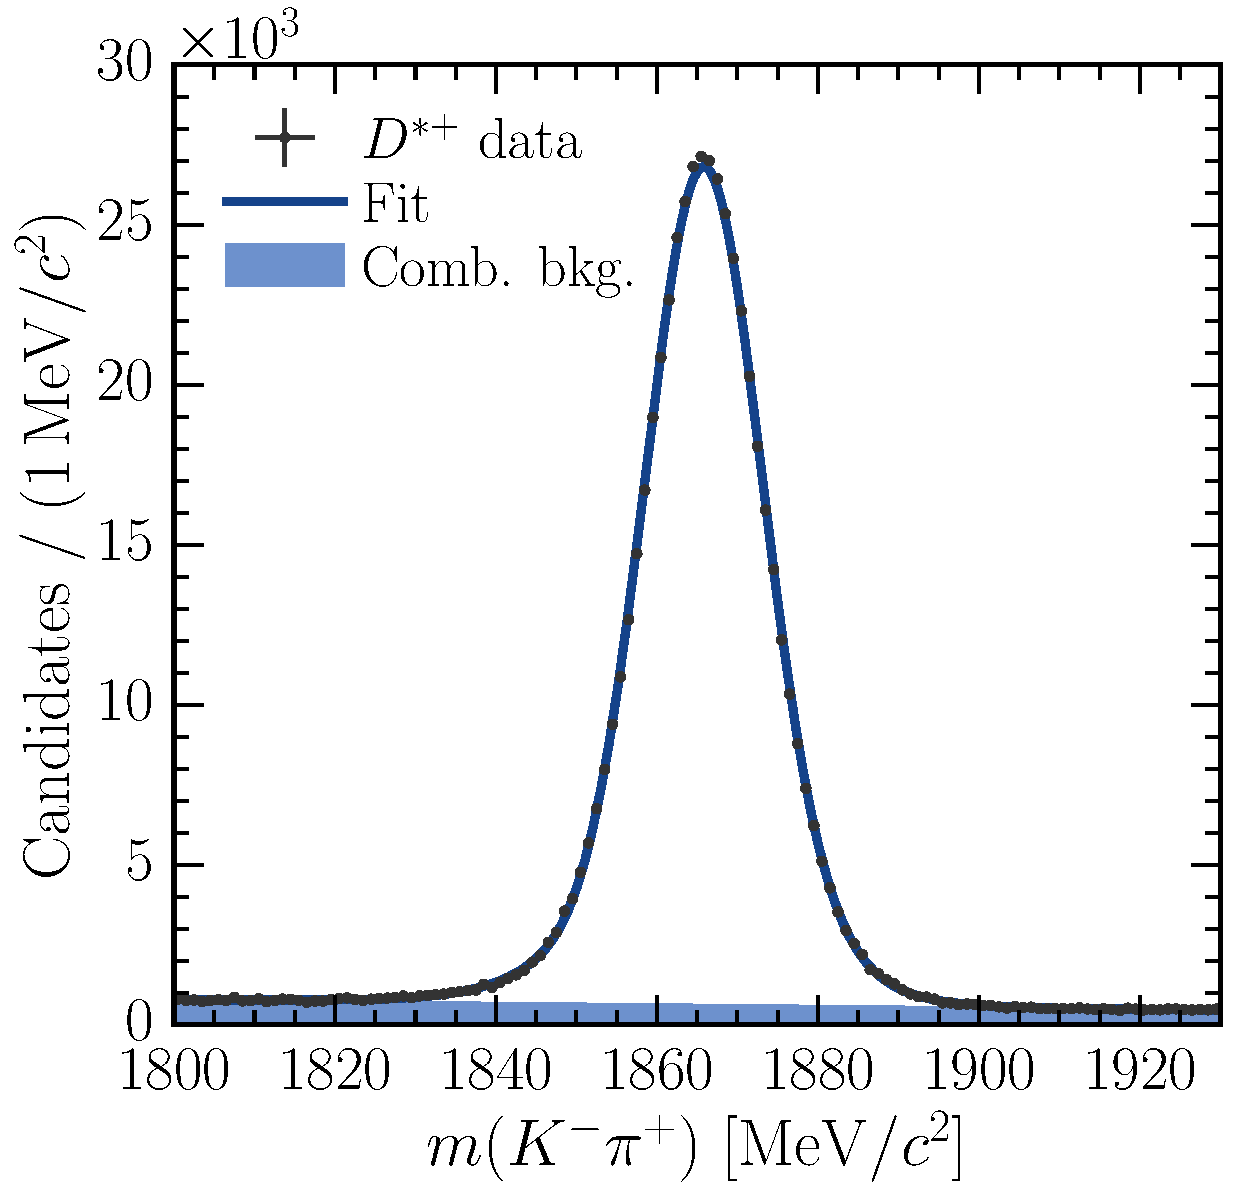
\includegraphics[width=\textwidth]{production/fitting/DstToD0pi_D0ToKpi_mass_fit_pT_integrated_y_integrated}
    \caption{\PDzero mass}
    \label{fig:prod:fitting:DstToD0pi_D0ToKpi:mass}
  \end{subfigure}
  \begin{subfigure}[b]{0.5\textwidth}
    \centering
    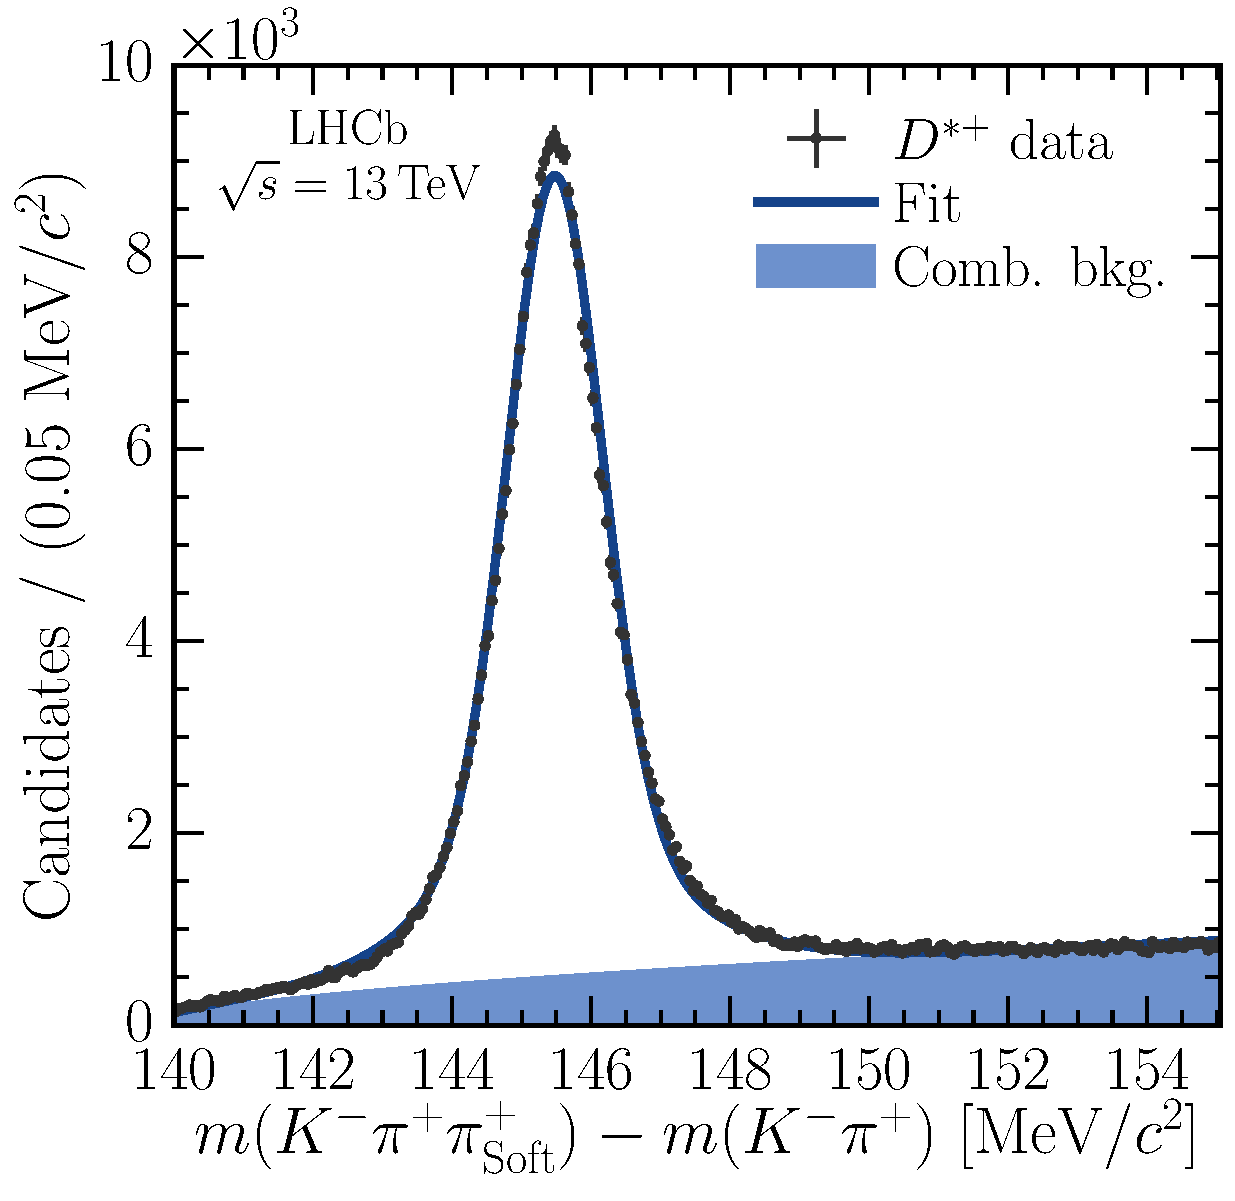
\includegraphics[width=\textwidth]{production/fitting/DstToD0pi_D0ToKpi_delta_mass_fit_pT_integrated_y_integrated}
    \caption{Delta mass}
    \label{fig:prod:fitting:DstToD0pi_D0ToKpi:delta_mass}
  \end{subfigure}
  \begin{subfigure}[b]{0.5\textwidth}
    \centering
    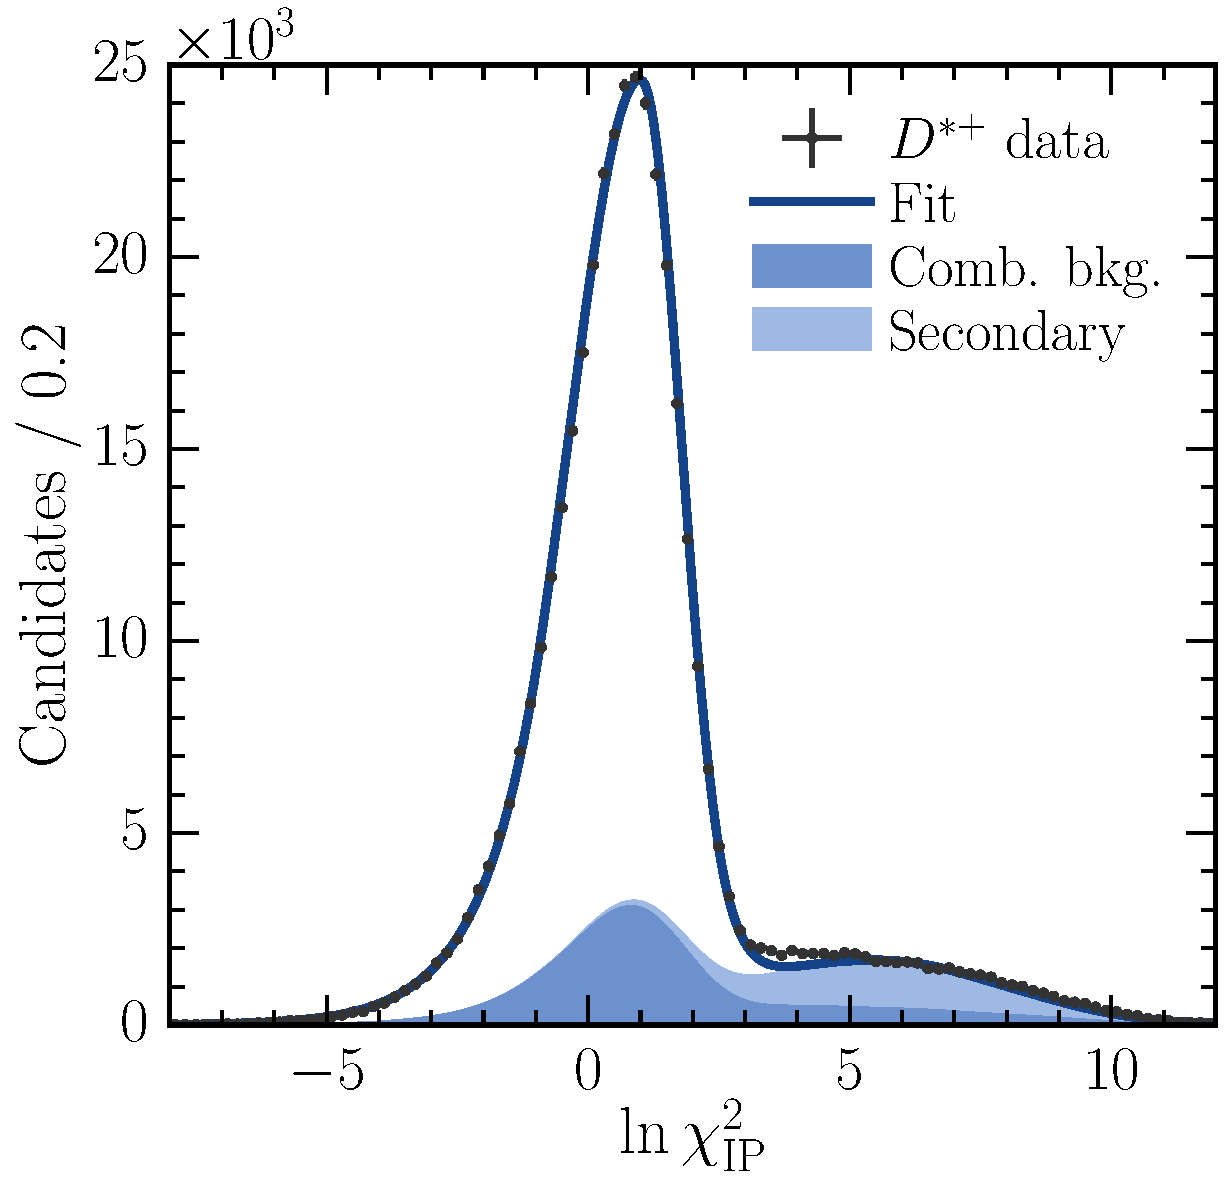
\includegraphics[width=\textwidth]{production/fitting/DstToD0pi_D0ToKpi_ipchisq_fit_pT_integrated_y_integrated}
    \caption{\lnipchisq}
    \label{fig:prod:fitting:DstToD0pi_D0ToKpi:ipchisq}
  \end{subfigure}
  \caption{%
    Distributions for fully selected \PDstarp\ candidates, with \DzToKpi: 
    \PDzero\ invariant mass 
    (\subref*{fig:prod:fitting:DstToD0pi_D0ToKpi:mass}); $\deltam = m(\PDstarp) 
    - m(\PDzero)$ (\subref*{fig:prod:fitting:DstToD0pi_D0ToKpi:delta_mass}) for 
    a mass window of $\pm\SI{20}{\MeVcc}$ around the nominal \PDzero mass; and 
    \PDzero\ \lnipchisq\ (\subref*{fig:prod:fitting:DstToD0pi_D0ToKpi:ipchisq}) 
    with an additional mass window of $\pm\SI{3}{\MeVcc}$ around the nominal 
    \deltam\ value.
    The sum of the simultaneous likelihood fits in each \pTy\ bin is shown, 
    with components as indicated in the legends.
  }
  \label{fig:prod:fitting:DstToD0pi_D0ToKpi}
\end{figure}

\begin{table}
  \caption{%
    Prompt signal yields in the fully selected dataset, summed over all
    \pTy\ bins in which a measurement is made.
  }
  \label{tab:prod:fitting:integrated}
  \centering
  \begin{tabular}{lr}
  \toprule
  Hadron   & Prompt signal yield              \\
  \midrule
  \PDzero  & $(25.77 \pm 0.02) \times 10^{5}$ \\
  \PDplus  & $(19.74 \pm 0.02) \times 10^{5}$ \\
  \PDsplus & $(11.32 \pm 0.04) \times 10^{4}$ \\
  \PDstarp & $(30.12 \pm 0.06) \times 10^{4}$ \\
  \bottomrule
\end{tabular}

\end{table}

\begin{figure}
  \begin{subfigure}[b]{0.5\textwidth}
    \centering
    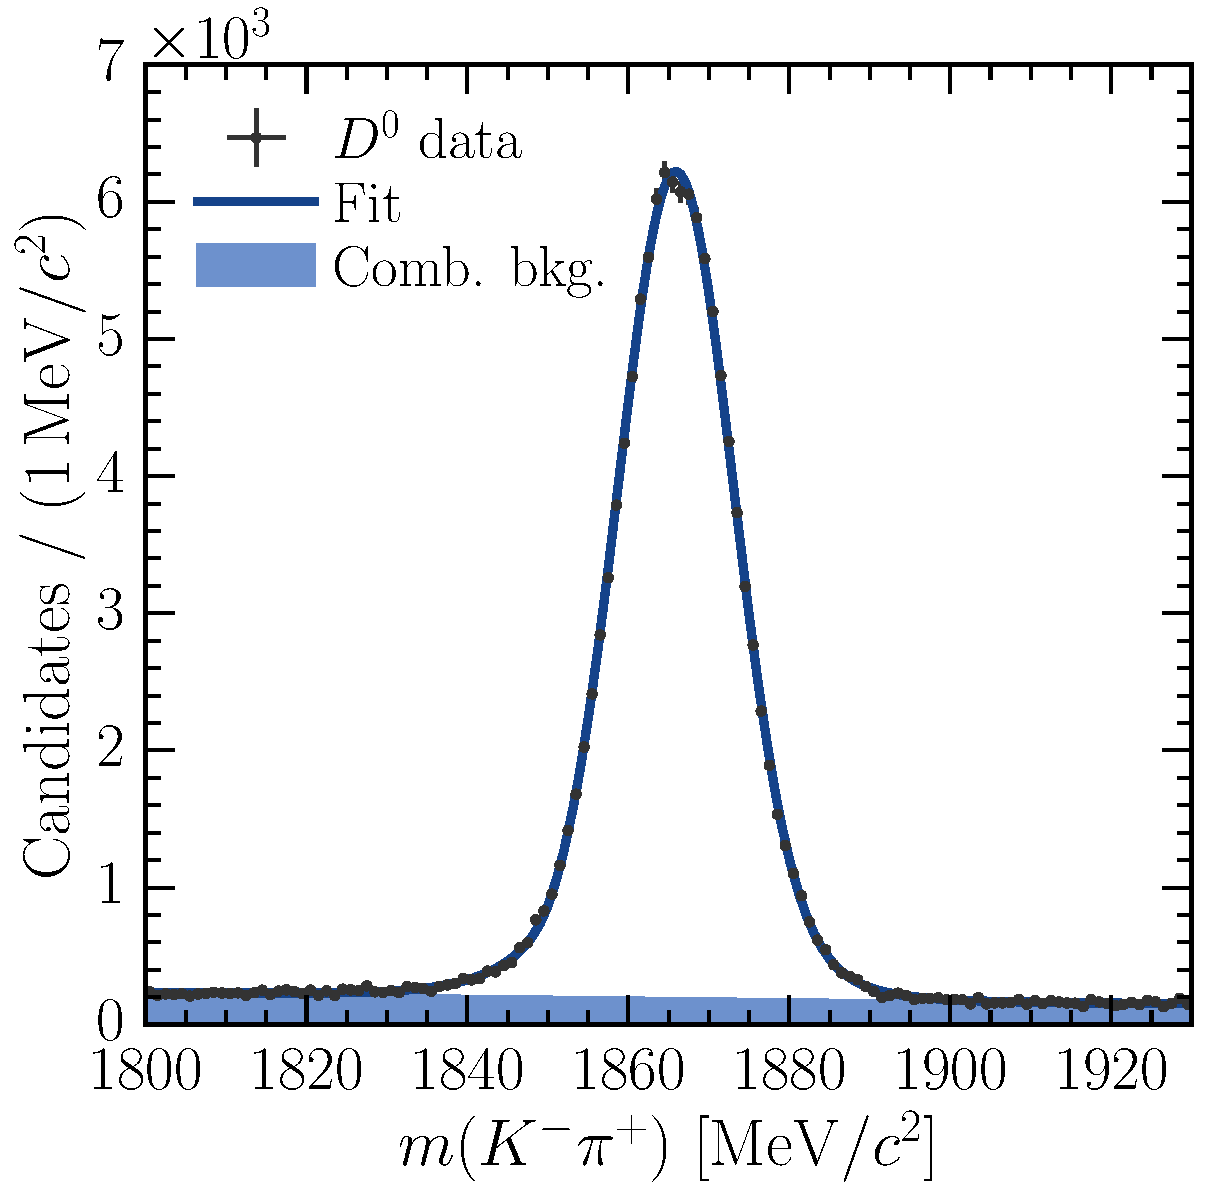
\includegraphics[width=\textwidth]{production/fitting/D0ToKpi_mass_fit_pT_3_y_2}
    \caption{Mass}
    \label{fig:prod:fitting:D0ToKpi:mass_high_sig}
  \end{subfigure}
  \begin{subfigure}[b]{0.5\textwidth}
    \centering
    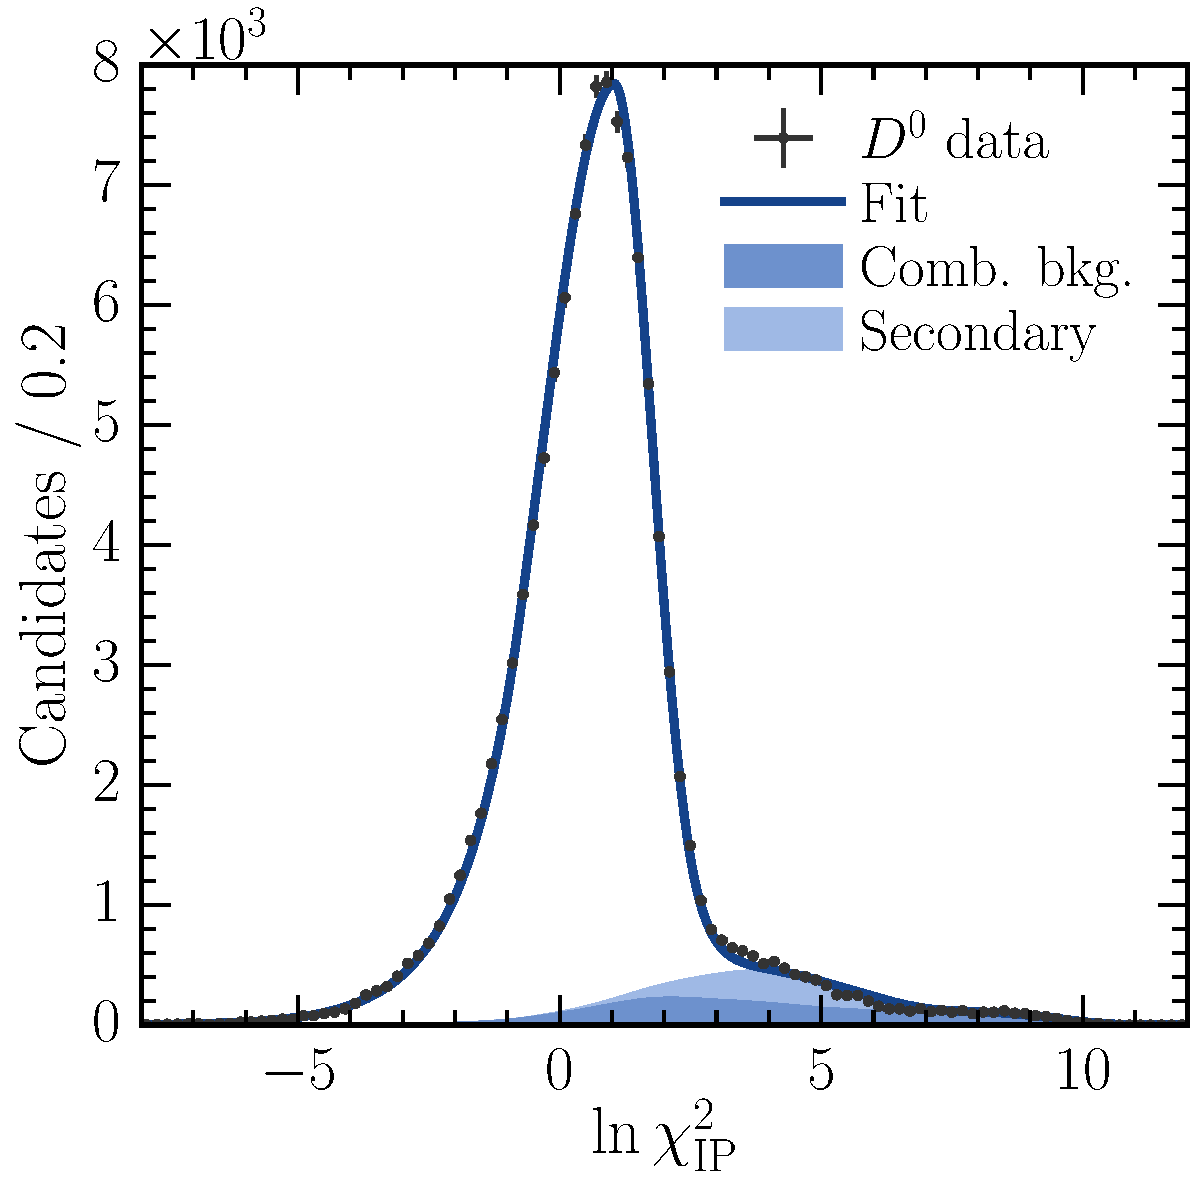
\includegraphics[width=\textwidth]{production/fitting/D0ToKpi_ipchisq_fit_pT_3_y_2}
    \caption{\lnipchisq}
    \label{fig:prod:fitting:D0ToKpi:ipchisq_high_sig}
  \end{subfigure}
  \begin{subfigure}[b]{0.5\textwidth}
    \centering
    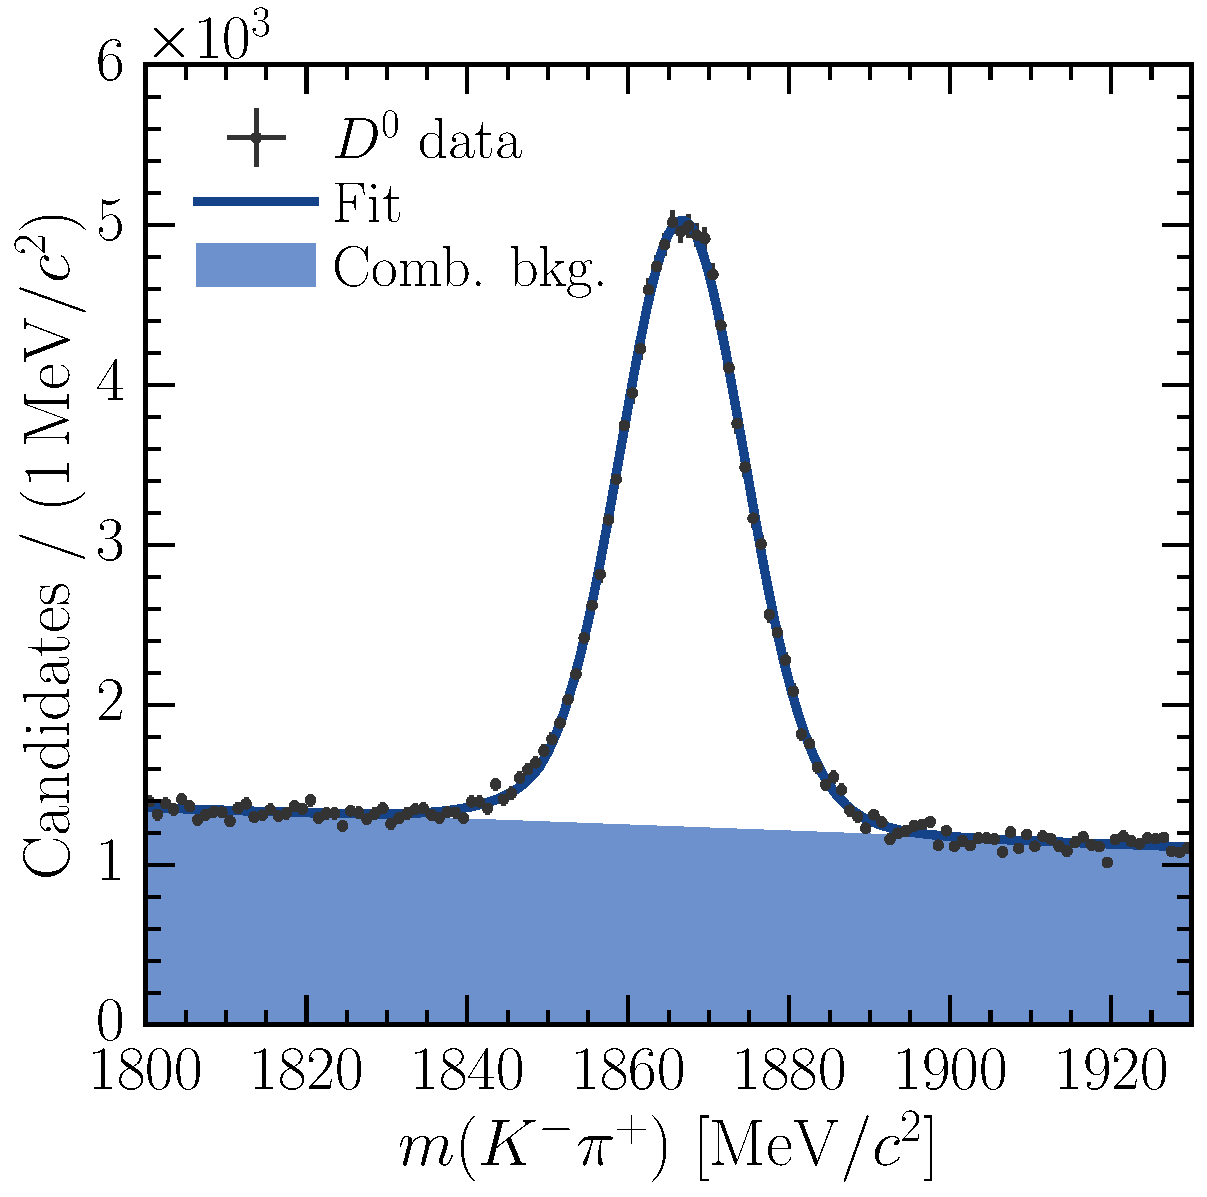
\includegraphics[width=\textwidth]{production/fitting/D0ToKpi_mass_fit_pT_0_y_3}
    \caption{Mass}
    \label{fig:prod:fitting:D0ToKpi:mass_high_bkg}
  \end{subfigure}
  \begin{subfigure}[b]{0.5\textwidth}
    \centering
    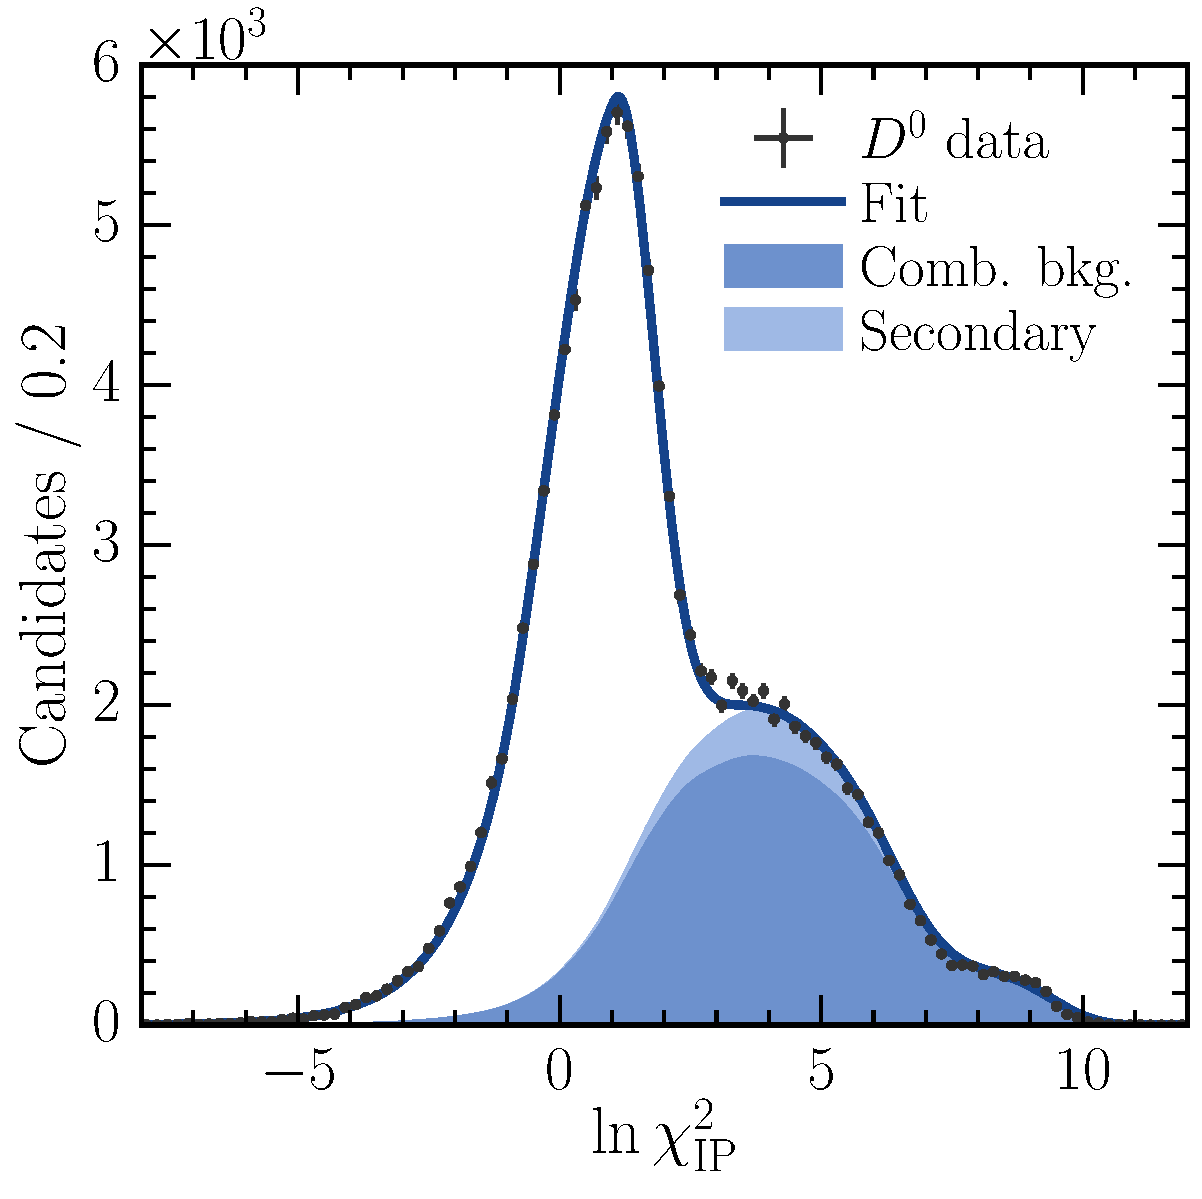
\includegraphics[width=\textwidth]{production/fitting/D0ToKpi_ipchisq_fit_pT_0_y_3}
    \caption{\lnipchisq}
    \label{fig:prod:fitting:D0ToKpi:ipchisq_high_bkg}
  \end{subfigure}
  \caption{%
    Distributions for fully selected \DzToKpi\ candidates: \PDzero\ invariant 
    mass (\subref*{fig:prod:fitting:D0ToKpi:mass_high_sig} and 
    \subref*{fig:prod:fitting:D0ToKpi:mass_high_bkg}); and \PDzero\ \lnipchisq\ 
    (\subref*{fig:prod:fitting:D0ToKpi:ipchisq_high_sig} and 
    \subref*{fig:prod:fitting:D0ToKpi:ipchisq_high_bkg}) for a mass window of 
    $\pm\SI{20}{\MeVcc}$ around the nominal \PDzero mass.
    The top Figures (\subref*{fig:prod:fitting:D0ToKpi:mass_high_sig} and 
    \subref*{fig:prod:fitting:D0ToKpi:ipchisq_high_sig}) show the data and fits 
    in the region \pTyrange{2}{2.5}{3}{3.5}, whilst the bottom Figures 
    (\subref*{fig:prod:fitting:D0ToKpi:mass_high_bkg} and 
    \subref*{fig:prod:fitting:D0ToKpi:ipchisq_high_bkg}) show the data and fits 
    in the \pTyrange{0}{1}{3.5}{4} region.
  }
  \label{fig:prod:fitting:D0ToKpi:sig_bkg}
\end{figure}

\begin{figure}
  \begin{subfigure}[b]{0.5\textwidth}
    \centering
    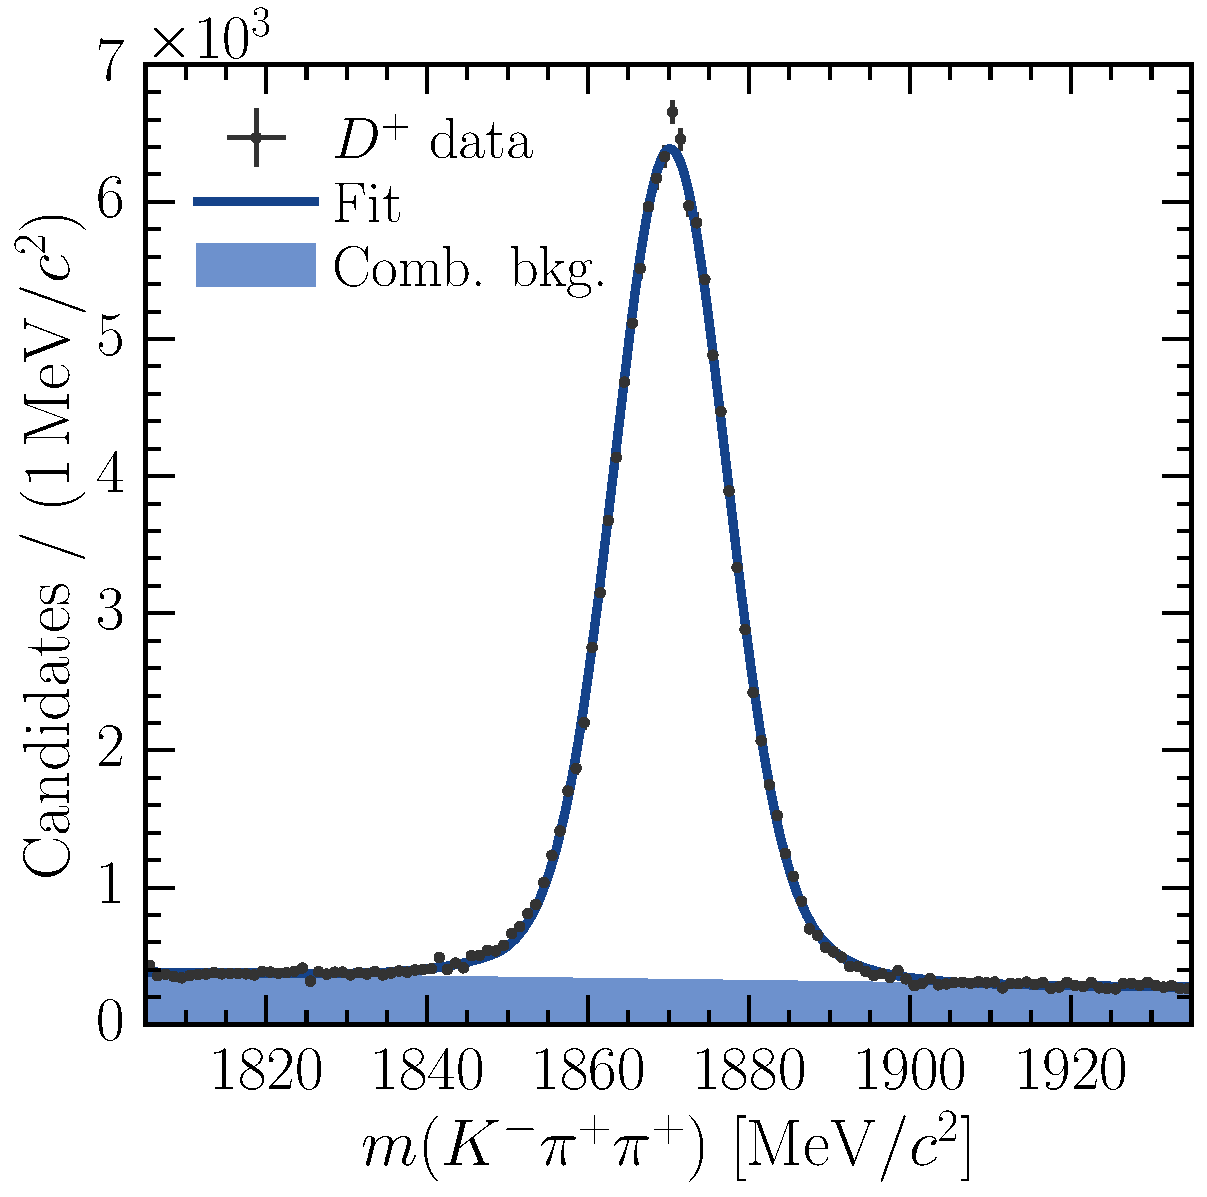
\includegraphics[width=\textwidth]{production/fitting/DpToKpipi_mass_fit_pT_4_y_2}
    \caption{Mass}
    \label{fig:prod:fitting:DpToKpipi:mass_high_sig}
  \end{subfigure}
  \begin{subfigure}[b]{0.5\textwidth}
    \centering
    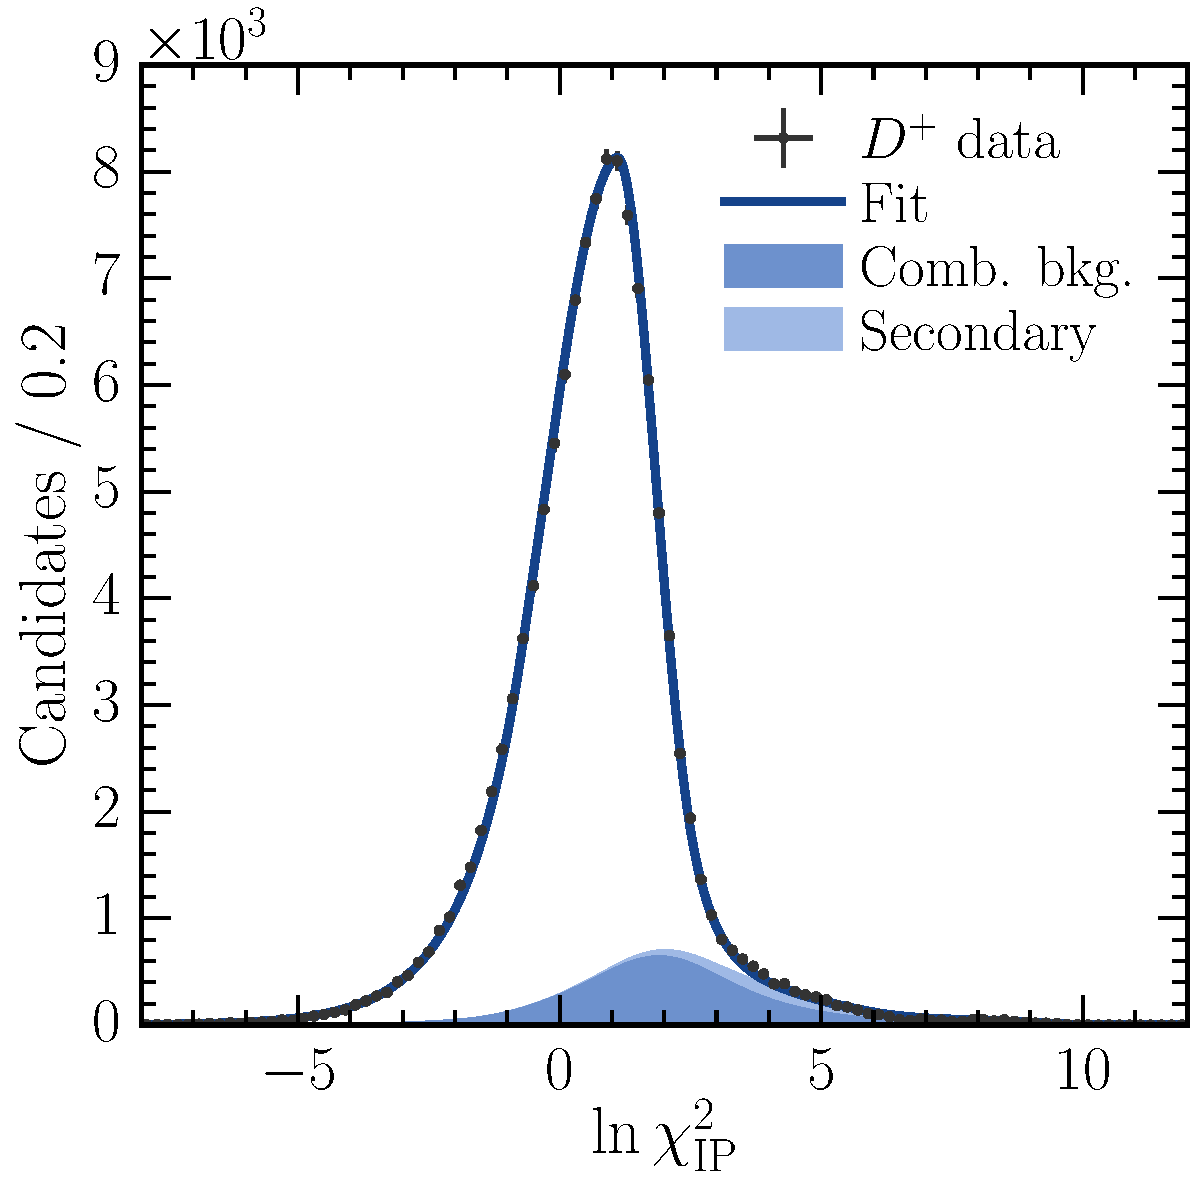
\includegraphics[width=\textwidth]{production/fitting/DpToKpipi_ipchisq_fit_pT_4_y_2}
    \caption{\lnipchisq}
    \label{fig:prod:fitting:DpToKpipi:ipchisq_high_sig}
  \end{subfigure}
  \begin{subfigure}[b]{0.5\textwidth}
    \centering
    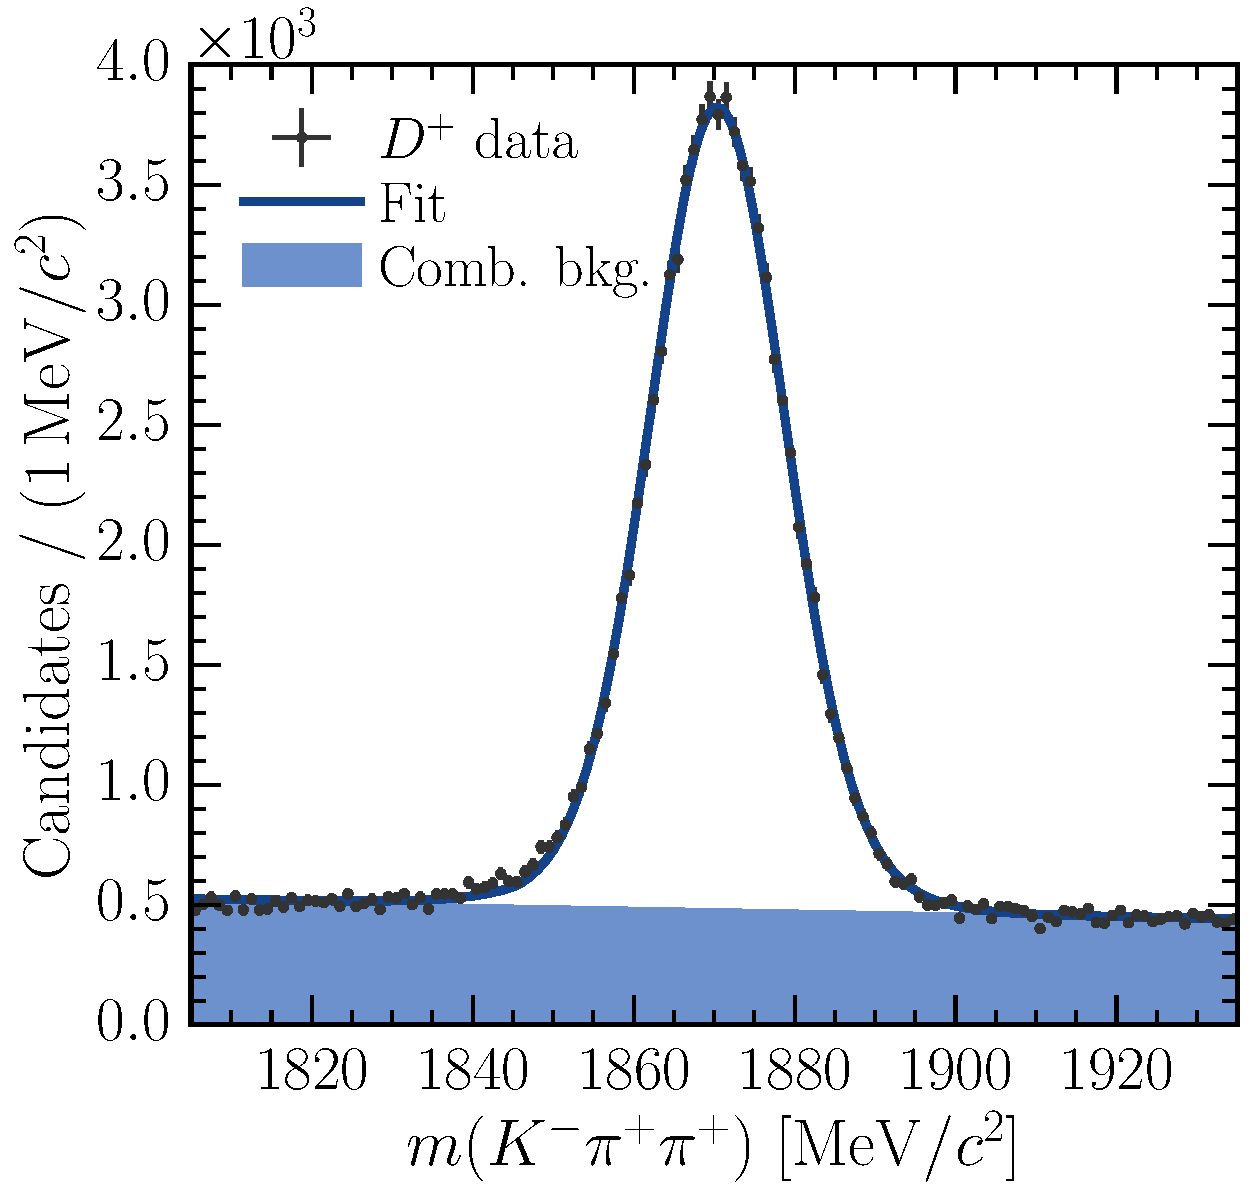
\includegraphics[width=\textwidth]{production/fitting/DpToKpipi_mass_fit_pT_3_y_3}
    \caption{Mass}
    \label{fig:prod:fitting:DpToKpipi:mass_high_bkg}
  \end{subfigure}
  \begin{subfigure}[b]{0.5\textwidth}
    \centering
    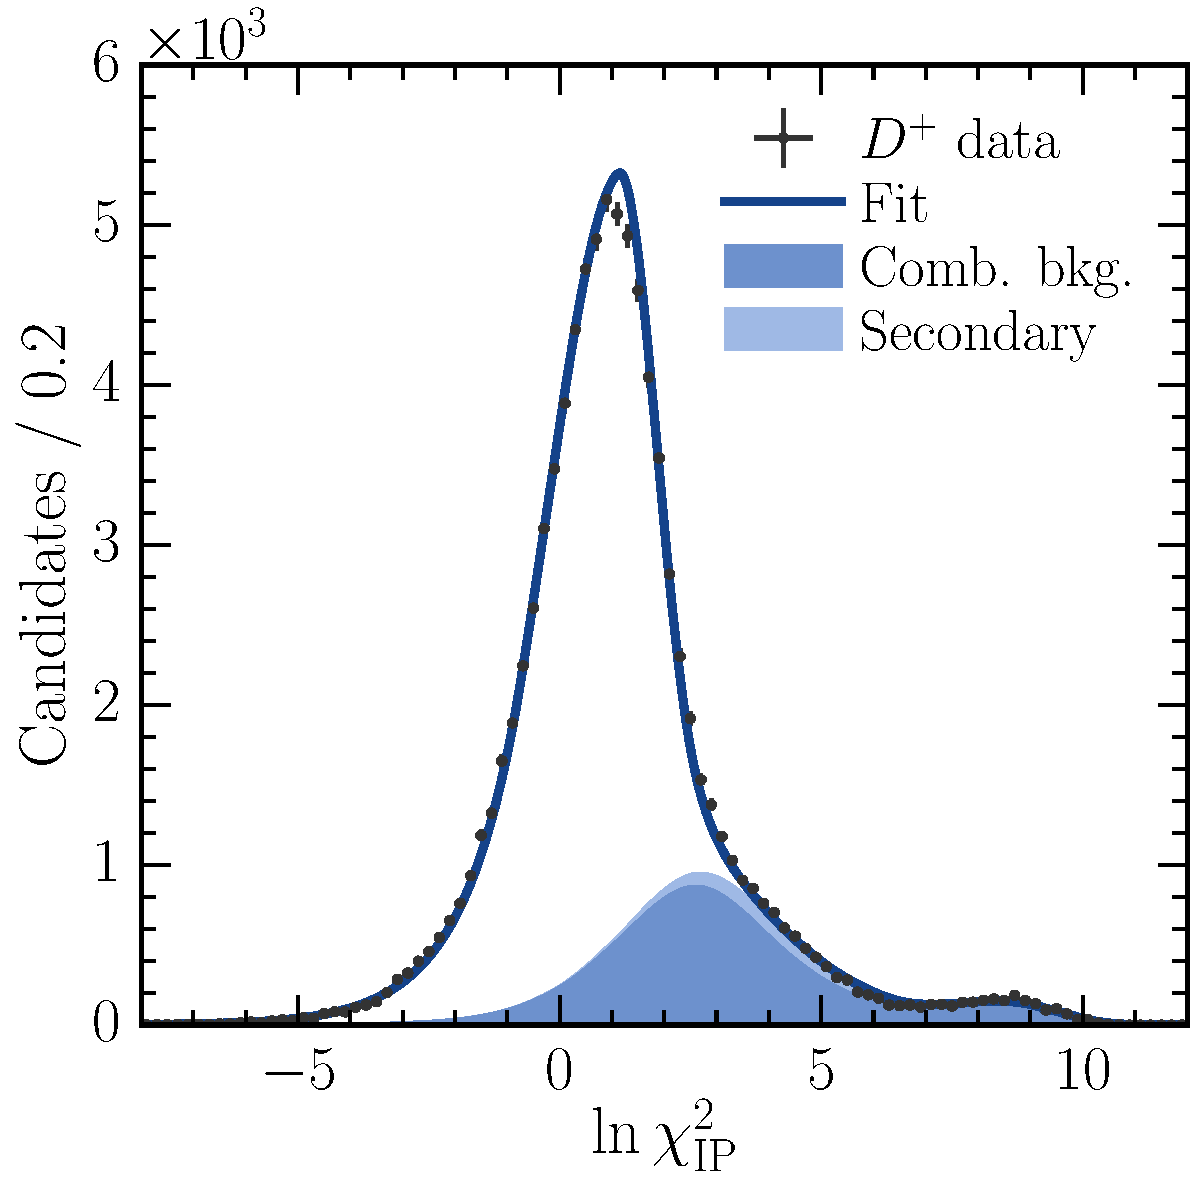
\includegraphics[width=\textwidth]{production/fitting/DpToKpipi_ipchisq_fit_pT_3_y_3}
    \caption{\lnipchisq}
    \label{fig:prod:fitting:DpToKpipi:ipchisq_high_bkg}
  \end{subfigure}
  \caption{%
    Distributions for fully selected \DpToKpipi\ candidates: \PDplus\ invariant 
    mass (\subref*{fig:prod:fitting:DpToKpipi:mass_high_sig} and 
    \subref*{fig:prod:fitting:DpToKpipi:mass_high_bkg}); and \PDplus\ 
    \lnipchisq\ (\subref*{fig:prod:fitting:DpToKpipi:ipchisq_high_sig} and 
    \subref*{fig:prod:fitting:DpToKpipi:ipchisq_high_bkg}) for a mass window of 
    $\pm\SI{20}{\MeVcc}$ around the nominal \PDplus mass.
    The top Figures (\subref*{fig:prod:fitting:DpToKpipi:mass_high_sig} and 
    \subref*{fig:prod:fitting:DpToKpipi:ipchisq_high_sig}) show the data and 
    fits in the region \pTyrange{2.5}{3}{3}{3.5}, whilst the bottom Figures 
    (\subref*{fig:prod:fitting:DpToKpipi:mass_high_bkg} and 
    \subref*{fig:prod:fitting:DpToKpipi:ipchisq_high_bkg}) show the data and 
    fits in the \pTyrange{2}{2.5}{3.5}{4} region.
  }
  \label{fig:prod:fitting:DpToKpipi:sig_bkg}
\end{figure}

\begin{figure}
  \begin{subfigure}[b]{0.5\textwidth}
    \centering
    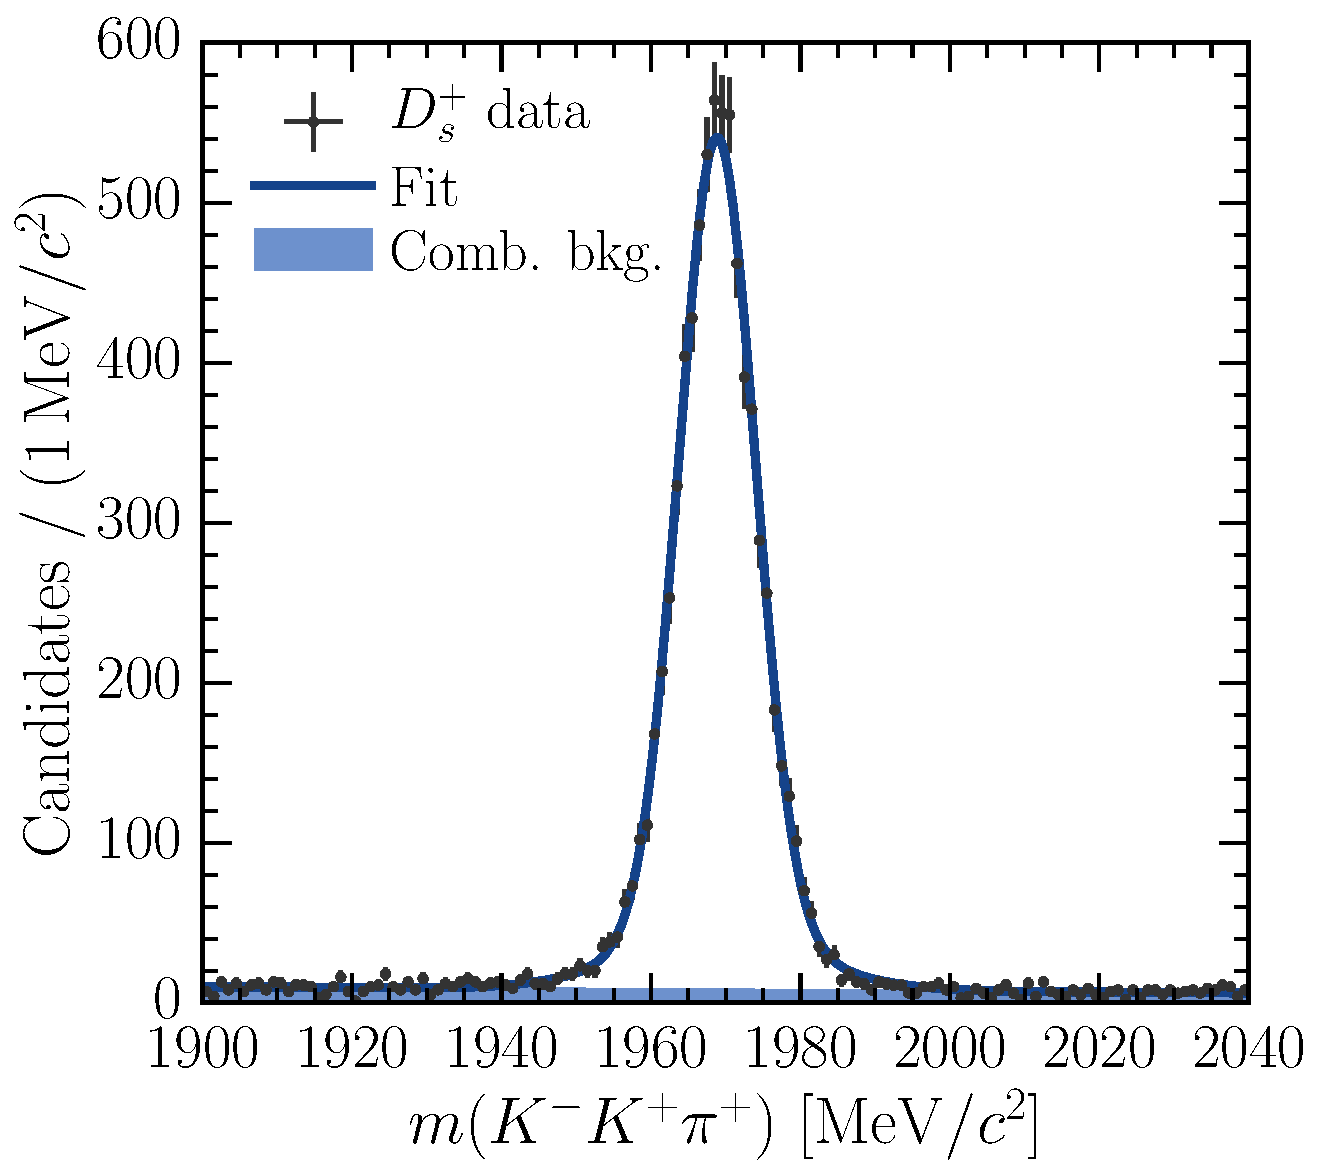
\includegraphics[width=\textwidth]{production/fitting/DsToKKpi_mass_fit_pT_6_y_1}
    \caption{Mass}
    \label{fig:prod:fitting:DsToKKpi:mass_high_sig}
  \end{subfigure}
  \begin{subfigure}[b]{0.5\textwidth}
    \centering
    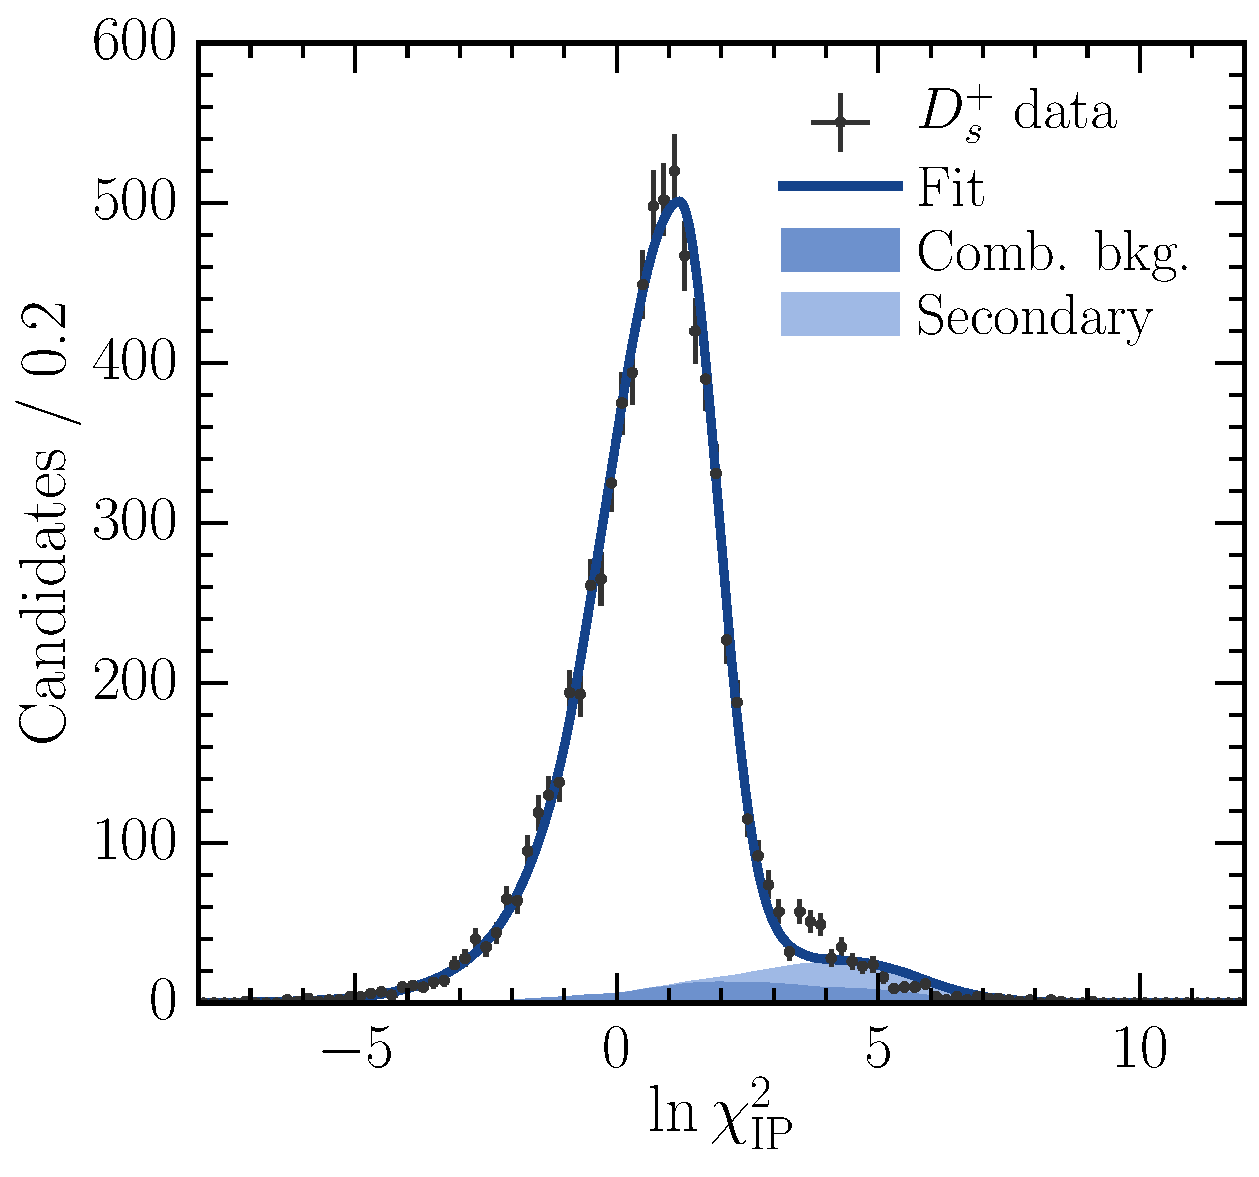
\includegraphics[width=\textwidth]{production/fitting/DsToKKpi_ipchisq_fit_pT_6_y_1}
    \caption{\lnipchisq}
    \label{fig:prod:fitting:DsToKKpi:ipchisq_high_sig}
  \end{subfigure}
  \begin{subfigure}[b]{0.5\textwidth}
    \centering
    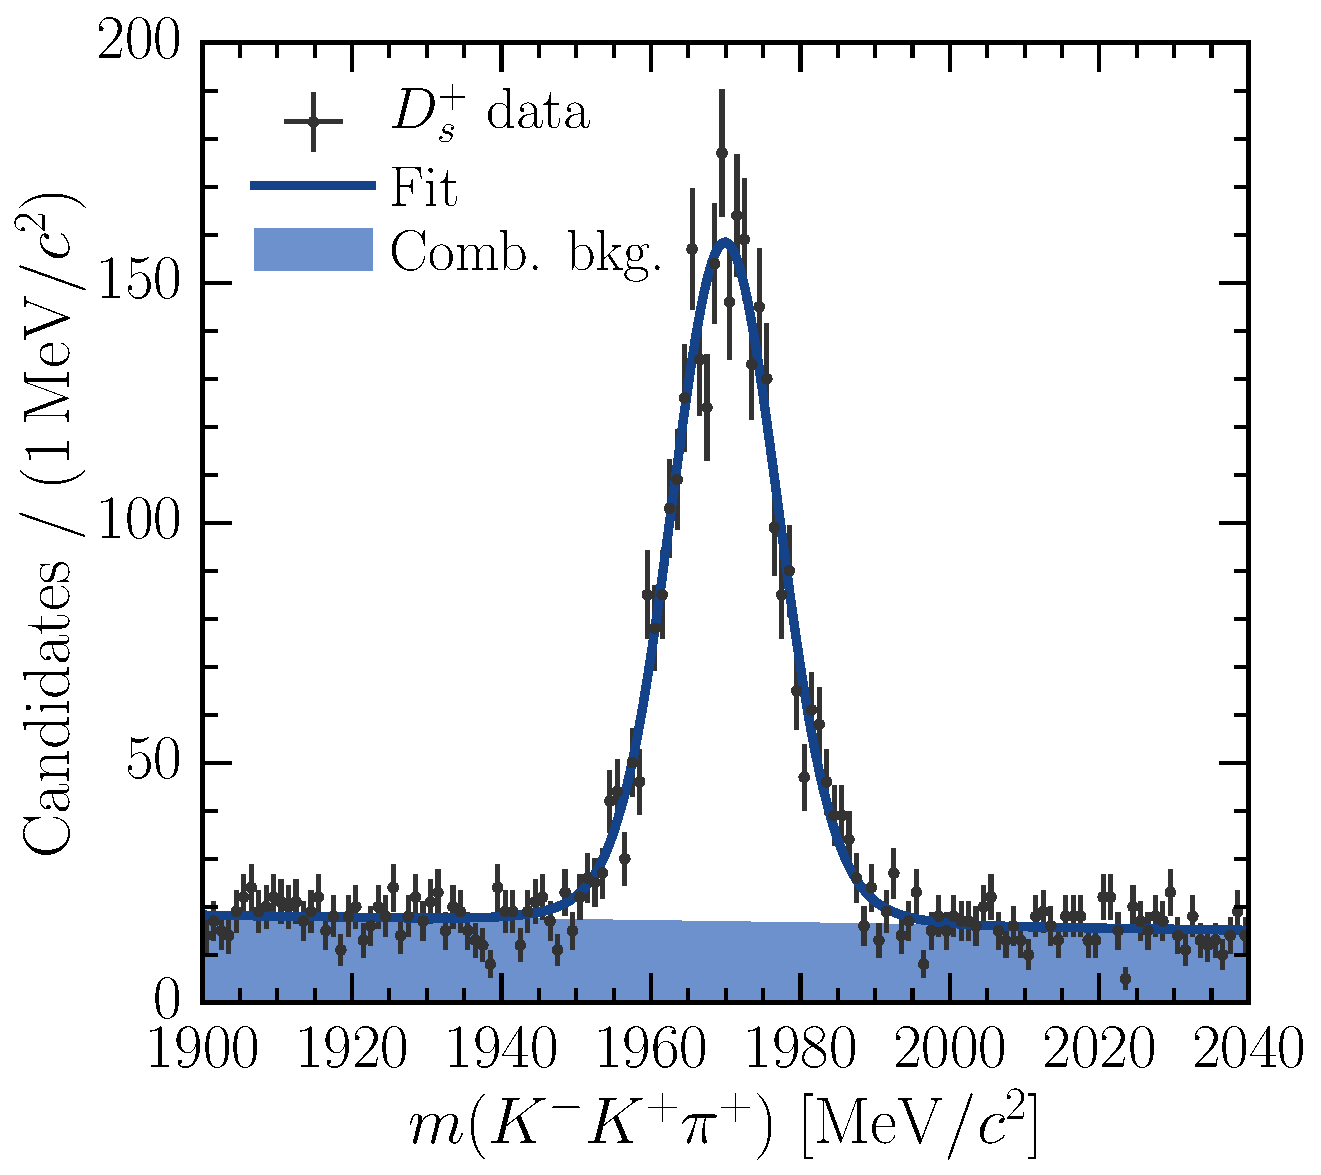
\includegraphics[width=\textwidth]{production/fitting/DsToKKpi_mass_fit_pT_2_y_3}
    \caption{Mass}
    \label{fig:prod:fitting:DsToKKpi:mass_high_bkg}
  \end{subfigure}
  \begin{subfigure}[b]{0.5\textwidth}
    \centering
    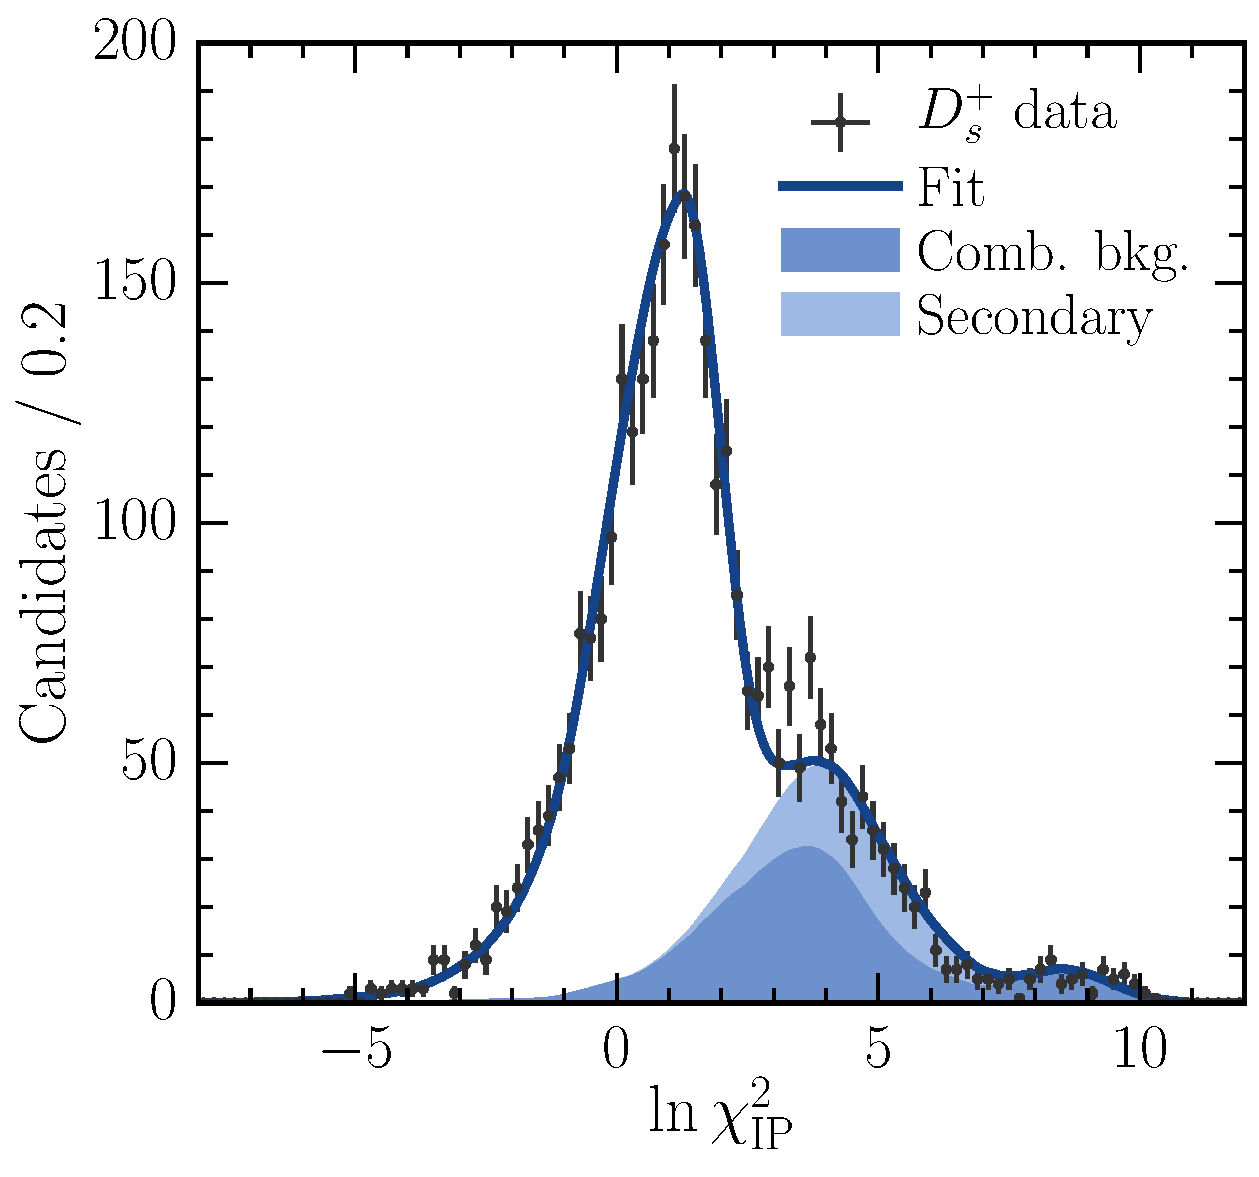
\includegraphics[width=\textwidth]{production/fitting/DsToKKpi_ipchisq_fit_pT_2_y_3}
    \caption{\lnipchisq}
    \label{fig:prod:fitting:DsToKKpi:ipchisq_high_bkg}
  \end{subfigure}
  \caption{%
    Distributions for fully selected \DspTophipi\ candidates: \PDsplus\ 
    invariant mass (\subref*{fig:prod:fitting:DsToKKpi:mass_high_sig} and 
    \subref*{fig:prod:fitting:DsToKKpi:mass_high_bkg}); and \PDsplus\ 
    \lnipchisq\ (\subref*{fig:prod:fitting:DsToKKpi:ipchisq_high_sig} and 
    \subref*{fig:prod:fitting:DsToKKpi:ipchisq_high_bkg}) for a mass window of 
    $\pm\SI{20}{\MeVcc}$ around the nominal \PDsplus mass.
    The top Figures (\subref*{fig:prod:fitting:DsToKKpi:mass_high_sig} and 
    \subref*{fig:prod:fitting:DsToKKpi:ipchisq_high_sig}) show the data and 
    fits in the region \pTyrange{4}{5}{2.5}{3}, whilst the bottom Figures 
    (\subref*{fig:prod:fitting:DsToKKpi:mass_high_bkg} and 
    \subref*{fig:prod:fitting:DsToKKpi:ipchisq_high_bkg}) show the data and 
    fits in the \pTyrange{2}{2.5}{3.5}{4} region.
  }
  \label{fig:prod:fitting:DsToKKpi:sig_bkg}
\end{figure}

\begin{figure}
  \begin{subfigure}[b]{0.5\textwidth}
    \centering
    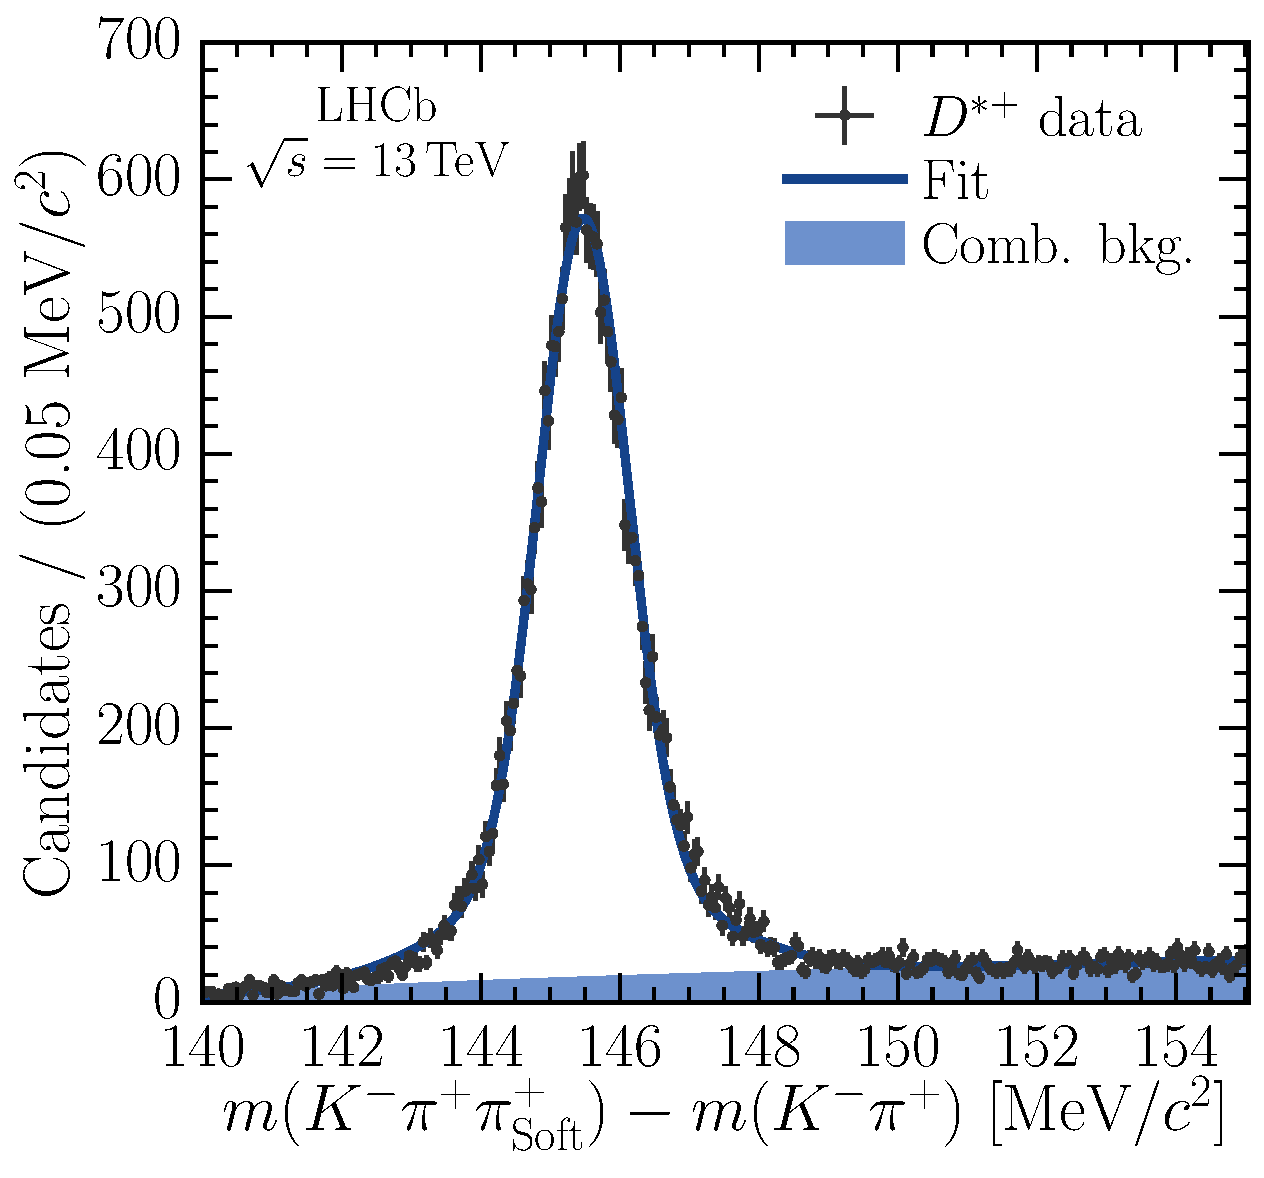
\includegraphics[width=\textwidth]{production/fitting/DstToD0pi_D0ToKpi_delta_mass_fit_pT_7_y_2}
    \caption{Delta mass}
    \label{fig:prod:fitting:DstToD0pi_D0ToKpi:delta_mass_high_sig}
  \end{subfigure}
  \begin{subfigure}[b]{0.5\textwidth}
    \centering
    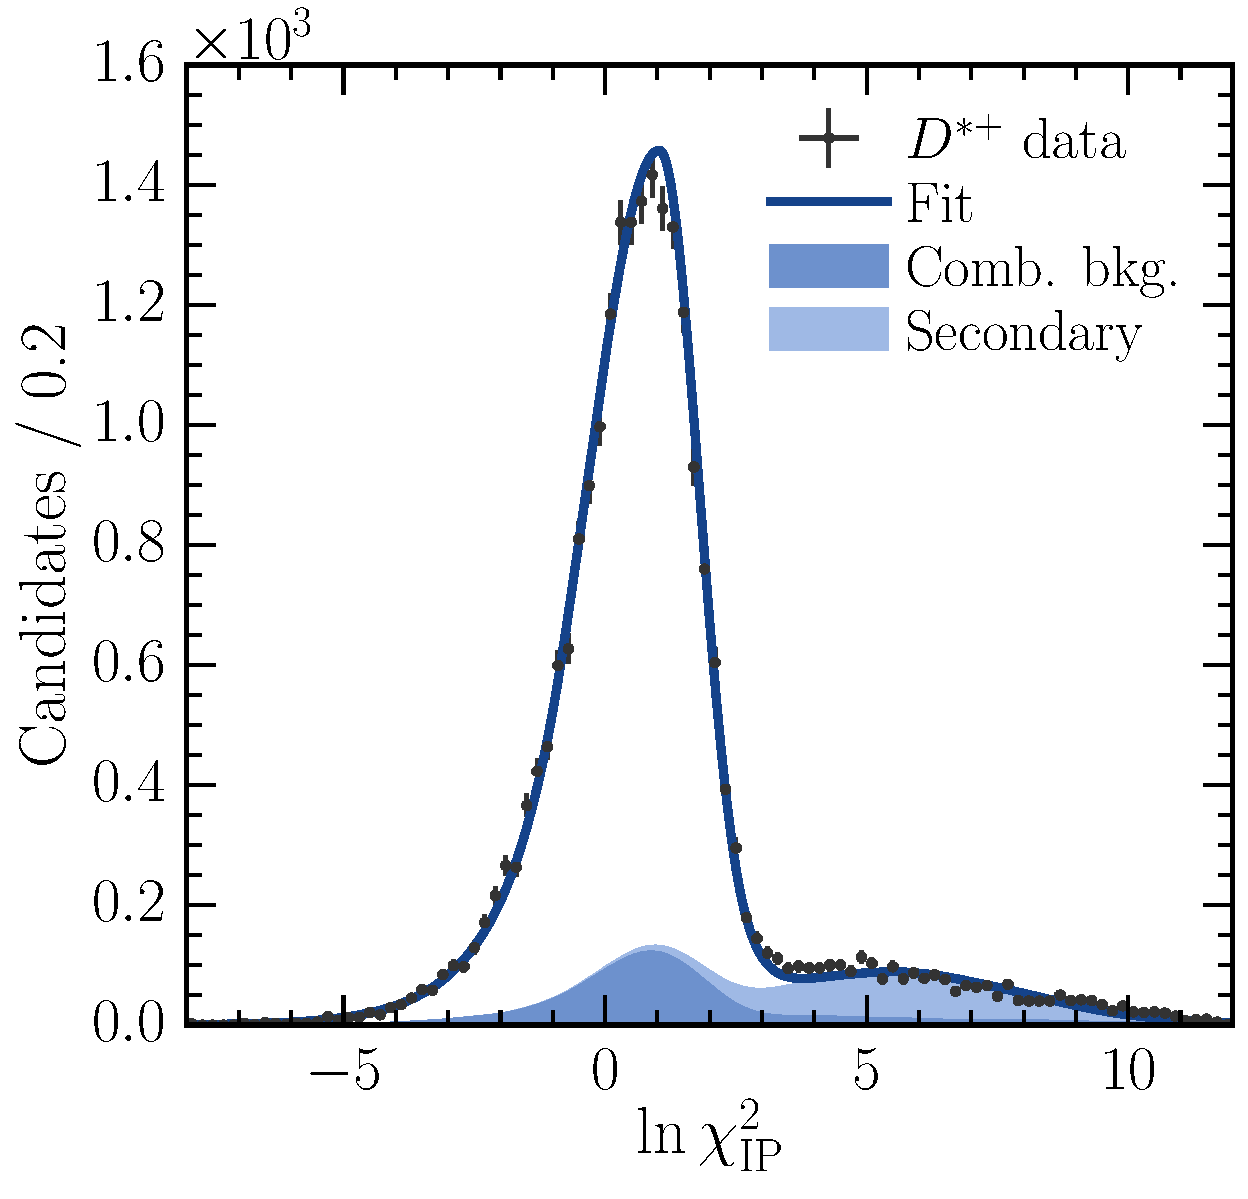
\includegraphics[width=\textwidth]{production/fitting/DstToD0pi_D0ToKpi_ipchisq_fit_pT_7_y_2}
    \caption{\lnipchisq}
    \label{fig:prod:fitting:DstToD0pi_D0ToKpi:ipchisq_high_sig}
  \end{subfigure}
  \begin{subfigure}[b]{0.5\textwidth}
    \centering
    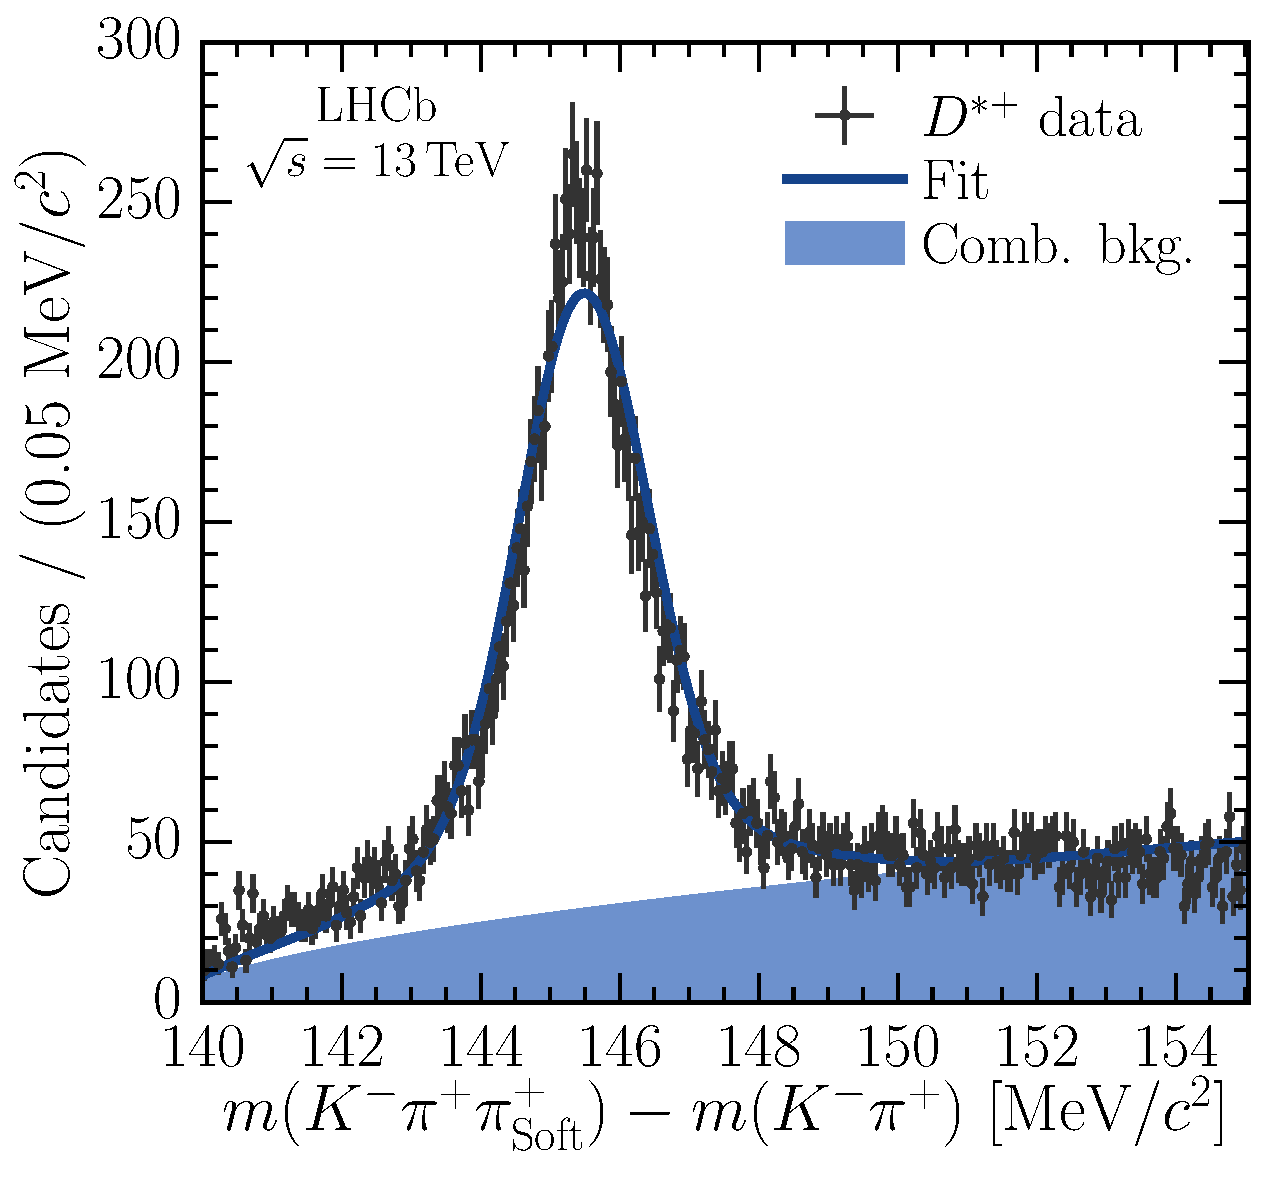
\includegraphics[width=\textwidth]{production/fitting/DstToD0pi_D0ToKpi_delta_mass_fit_pT_2_y_3}
    \caption{Delta mass}
    \label{fig:prod:fitting:DstToD0pi_D0ToKpi:delta_mass_high_bkg}
  \end{subfigure}
  \begin{subfigure}[b]{0.5\textwidth}
    \centering
    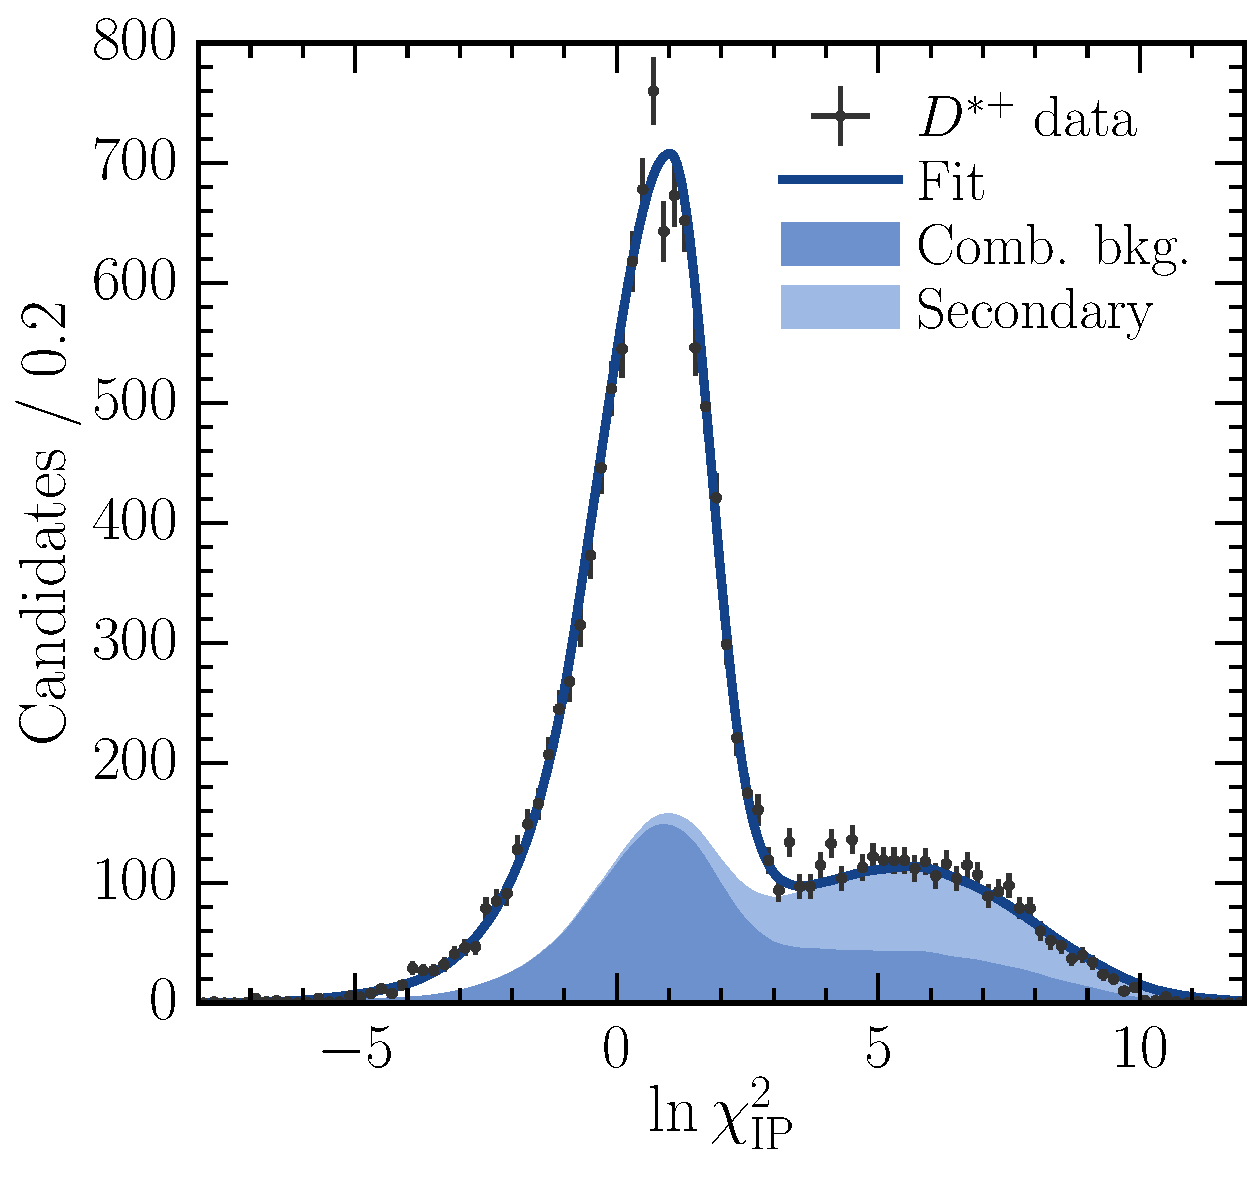
\includegraphics[width=\textwidth]{production/fitting/DstToD0pi_D0ToKpi_ipchisq_fit_pT_2_y_3}
    \caption{\lnipchisq}
    \label{fig:prod:fitting:DstToD0pi_D0ToKpi:ipchisq_high_bkg}
  \end{subfigure}
  \caption{%
    Distributions for fully selected \DstToDzpi, with \DzToKpi, candidates: 
    $\deltam = m(\PDstarp) - m(\PDzero)$ 
    (\subref*{fig:prod:fitting:DstToD0pi_D0ToKpi:delta_mass_high_sig} and 
    \subref*{fig:prod:fitting:DstToD0pi_D0ToKpi:delta_mass_high_bkg}) for a 
    mass window of $\pm\SI{20}{\MeVcc}$ around the nominal \PDzero mass; and 
    \PDzero\ \lnipchisq\ 
    (\subref*{fig:prod:fitting:DstToD0pi_D0ToKpi:ipchisq_high_sig} and 
    \subref*{fig:prod:fitting:DstToD0pi_D0ToKpi:ipchisq_high_bkg}) with an 
    additional mass window of $\pm\SI{3}{\MeVcc}$ around the nominal 
    \PDstarp-\PDzero\ mass difference.
    The top Figures 
    (\subref*{fig:prod:fitting:DstToD0pi_D0ToKpi:delta_mass_high_sig} and 
    \subref*{fig:prod:fitting:DstToD0pi_D0ToKpi:ipchisq_high_sig}) show the 
    data and fits in the region \pTyrange{4}{5}{3}{3.5}, whilst the bottom 
    Figures (\subref*{fig:prod:fitting:DstToD0pi_D0ToKpi:delta_mass_high_bkg} 
    and \subref*{fig:prod:fitting:DstToD0pi_D0ToKpi:ipchisq_high_bkg}) show the 
    data and fits in the \pTyrange{1.5}{2}{3.5}{4} region.
  }
  \label{fig:prod:fitting:DstToD0pi_D0ToKpi:sig_bkg}
\end{figure}
